\documentclass[lualatex,12pt,a4paper]{article}
\usepackage{style/arpafvg}
\usepackage{caption,booktabs,siunitx,float,pdflscape}
\usepackage{natbib}
\usepackage{lscape}
\usepackage{placeins}
\usepackage{svg}

%\usepackage{draftwatermark}
%\SetWatermarkText{BOZZA}
%\SetWatermarkScale{1.2}

\begin{document}
\AddToShipoutPicture*{\BackgroundPic}
\title
{Effetti sulla matrice ambientale ARIA delle azioni di contenimento del COVID-19
 \\ 
\Large{Relazione tecnica}}
\author
{SOS Qualità dell'aria\\
 Centro regionale di modellistica ambientale (CRMA)\\
 IPAS Analisi chimiche ambientali
}
\date{giugno 2020}
\maketitle


\pagebreak
 \begingroup
   \hypersetup{hidelinks}
   \section*{Autori e ringraziamento}
   Edi Baiutti,
   Marco Bellini,
   Giovanni Bonafè,
   Andrea Mistaro,
   Francesco Montanari,
   Alessia Movia,
   Alessandra Petrini,
   Fulvio Stel,
   Arianna Tolloi,
   Marco Visintin
   
Questo lavoro è stato possibile anche grazie al progetto europeo LIFE-PREPAIR (LIFE15 IPE IT013, www.lifeprepair.eu), che opera per la qualità dell'aria nel Nord Italia e in Slovenia.

   \tableofcontents
   \listoffigures
   \listoftables
 \endgroup
\pagebreak

\section*{Sommario}\label{cap:intro}
\addcontentsline{toc}{section}{Sommario}
L'esperienza drammatica e dolorosa del \textit{lockdown} nazionale, necessario per il contenimento della diffusione dell'epidemia COVID-19, ha determinato condizioni di studio ambientale uniche, che consentono di valutare dal vivo gli effetti sull'ambiente del blocco di interi settori della società.
Questa condizione eccezionale - e auspicabilmente irripetibile - ha stimolato ARPA-FVG ad avviare la raccolta e l'analisi di una serie articolata di dati e informazioni sulla variazione della mobilità, sui livelli di inquinamento atmosferico, sulla riduzione delle emissioni degli inquinanti e sulle condizioni meteo che hanno interessato il periodo di blocco delle attività. 

Dal punto di vista emissivo questo lavoro ha mostrato come le misure emergenziali a livello regionale abbiano complessivamente prodotto soprattutto \textbf{riduzioni nelle emissioni} degli ossidi di azoto (circa -25\%), seguiti dall’anidride carbonica (circa -19\%) e dal monossido di carbonio (circa -16\%). Decisamente minori sono risultate le riduzioni nelle emissioni di ammoniaca (circa -3\%) e di materiale particolato (circa -8\%). L’entità di queste riduzioni è coerente con il fatto che le misure adottate nella nostra regione hanno agito soprattutto sui trasporti. 

La riduzione delle emissioni inquinanti ha determinato un \textbf{calo delle concentrazioni in aria} di \textbf{biossido di azoto} (circa -40\% rispetto agli anni precedenti), registrato dalle stazioni di monitoraggio regionali, che sostanzialmente ha anticipato di tre o quattro settimane la consueta diminuzione delle concentrazioni che si osserva in primavera. Altrettanto marcata, nelle postazioni per il monitoraggio degli impatti del traffico, è risultata anche la riduzione nelle concentrazioni del \textbf{benzene}.
Le \textbf{polveri sottili} hanno presentato un calo decisamente meno rilevante (pari o inferiore al 10\%) e fluttuazioni più marcate, determinate dalla meteorologia e da un evento di trasporto di polveri desertiche tra il 27 e il 29 marzo. 
L'\textbf{ozono} - inquinante fortemente legato alla radiazione solare e dunque molto variabile tra un anno e l'altro - non ha mostrato variazioni evidenti rispetto agli anni precedenti, anche se l’andamento giornaliero sembra indicarne un leggero aumento nel periodo del \textit{lockdown}. 

Oltre all’andamento delle concentrazioni dei singoli inquinanti, i dati raccolti nel periodo del \textit{lockdown} sono stati utilizzati anche per valutare l’efficacia di alcuni \textbf{indicatori combinati}, ottenuti facendo il rapporto tra diversi inquinanti. Questi indicatori sono meno soggetti agli effetti confondenti della meteorologia.
Il rapporto toluene/benzene ad esempio in corrispondenza del \textit{lockdown} è calato vistosamente, da valori tipici del traffico veicolare a valori caratteristici della combustione di legna. Il rapporto tra gli ossidi totali di azoto e il monossido di azoto ha evidenziato che gli effetti più marcati si sono manifestati in prossimità delle strade. Infine l'analisi granulometrica delle polveri sottili ha palesato il venir meno, durante il \textit{lockdown}, della risospensione della frazione grossolana del particolato, indotta dal transito di veicoli e usualmente registrata dalle stazioni di bordo strada.

L'analisi del contenuto di alcuni \textbf{metalli} nelle polveri sottili evidenzia un significativo calo di antimonio e rame, originati prevalentemente dall'usura dei freni dei veicoli. Viene inoltre confermata l'origine dal deserto vicino al Mar Caspio delle notevoli masse di polveri che hanno interessato tutta la regione tra il 27 e il 29 marzo.
Anche sul contenuto di \textbf{idrocarburi policiclici aromatici} (IPA) nel PM10 le azioni di contenimento del contagio hanno determinato effetti misurabili. Agendo in particolare sul traffico, hanno determinato la riduzione degli IPA associati ai trasporti, ma facendo risaltare quelli principalmente legati alla combustione domestica.

In conclusione dunque la riduzione delle emissioni dei trasporti porta evidenti benefici ambientali, ma per alcuni inquinanti non è sufficiente, neppure se applicata su grande scala e per lungo tempo. Per il miglioramento della qualità dell'aria sono necessarie perciò strategie che agiscano anche su altri settori, quali il riscaldamento domestico, l'agricoltura e l'industria.

\vfill
Questo lavoro è stato possibile anche grazie al progetto europeo LIFE-PREPAIR.
\pagebreak

\section*{Introduzione}\label{cap:intro}
\addcontentsline{toc}{section}{Introduzione}
Nei primi mesi del 2020 l'epidemia di COVID-19 ha coinvolto drammaticamente l'Italia. Per contenere il contagio, limitare l'impatto sul Sistema Sanitario Nazionale, ridurre i decessi, sono stati messi in atto provvedimenti di scala locale, regionale e nazionale. Tali provvedimenti hanno temporaneamente limitato la mobilità individuale e interrotto o ridotto alcune attività produttive e commerciali (Tab.\ref{tab:cronistoria}), determinando alcuni effetti sull'ambiente.

In questo rapporto analizziamo gli effetti ambientali registrati in Friuli Venezia Giulia relativi alla qualità dell'aria. Seguendo lo schema ``DPSIR''\footnote{schema Determinanti-Pressioni-Stato-Impatti-Risposte per la descrizione delle interazioni tra società e ambiente} approfondiamo 
\begin{itemize}
    \item \textbf{Determinanti}, cioè le variazioni nelle attività umane e dei parametri meteorologici più rilevanti dal punto di vista della qualità dell'aria;
    \item \textbf{Pressioni}, cioè le conseguenti variazioni nelle emissioni inquinanti in atmosfera;
    \item \textbf{Stato}, cioè come la composizione dell'aria che respiriamo è cambiata nelle settimane considerate.
\end{itemize}

Il periodo di studio copre febbraio e marzo 2020 per i determinanti antropici e le pressioni, estendendosi ad aprile per i determinanti meteorologici e gli indicatori di stato.

\begin{table}[ht]
    \centering
    \caption[Misure di contenimento del contagio e altri eventi rilevanti relativi a COVID-19]{Misure di contenimento del contagio e altri eventi rilevanti relativi a COVID-19 (aggiornamento: 4 giugno 2020)}
    \begin{tabular}{lll}
    \toprule
    \multicolumn{2}{l}{data} & descrizione \\
    \midrule
    \textbf{2019} &&\\
        dicembre    & 31 & le autorità cinesi riferiscono di un focolaio di polmoniti virali di origine ignota a Wuhan in Cina\\
 %   \midrule
    \textbf{2020} &&\\
        gennaio     & 30 & OMS dichiara l'emergenza sanitaria pubblica di interesse internazionale\\
                    & 31 & limitazioni ai voli da/per la Cina \\
                    &    & primi casi accertati COVID-19 in Italia\\
        febbraio    & 22 & ``zone rosse'' in alcuni Comuni (Lodigiano, Vo' Euganeo)\\
                    & 23 & chiusura delle scuole in alcune Regioni (incluso FVG)\\
                    & 25 & chiusura dei musei\\
        marzo       &  8 & \textit{lockdown} in Lombardia e in alcune aree di Veneto, Emilia-Romagna, Piemonte, Marche\\
                    &    & attenuazione delle limitazioni di mobilità e accesso nelle ``zone rosse''\\
                    &    & limitazione agli orari di apertura di alcuni esercizi \\
                    &  9 & \textit{lockdown} nazionale\\
                    &    & chiusura dei confini nazionali\\
                    &    & chiusura delle scuole in tutta Italia\\
                    & 11 & chiusura dei servizi pubblici\\
                    &    & OMS dichiara la pandemia\\
                    & 12 & chiusura di alcune categorie di esercizi (bar, ristoranti, ecc)\\
                    & 13 & resta attivo un solo aeroporto per ogni Regione\\
                    & 20 & chiusura dei parchi pubblici e dei cimiteri\\
                    & 23 & divieto di spostamento tra Comuni\\
                    &    & chiusura delle attività produttive non essenziali\\
        aprile      & 10 & riapertura di attività produttive che rispettino specifiche condizioni di sicurezza\\
                    & 11 & riapertura di alcuni esercizi (librerie, abbigliamento bambini, ecc)\\
        maggio      &  4 & maggiori possibilità di spostarsi tra Comuni e tra Regioni\\
                    &    & riapertura dei parchi pubblici\\
                    &    & riapertura di alcuni esercizi (\textit{take away})\\
                    &    & riapertura di alcune attività (manifatture, cantieri, ecc)\\
                    &    & incremento dei trasporti pubblici\\
                    & 18 & riapertura di alcuni esercizi (bar, ristoranti, ecc)\\
                    &    & possibilità di spostarsi all'interno della Regione\\
        giugno      &  3 & possibilità di spostarsi tra Regioni diverse\\
                    &    & riapertura dei confini nazionali agli altri Paesi UE\\
    \bottomrule                
    \end{tabular}
    \label{tab:cronistoria}
\end{table}



\FloatBarrier
\section{Determinanti}\label{cap:determinanti}
Innanzitutto sono stati analizzati i ``Determinanti'', cioè le attività umane (determinanti antropici) e il contesto meteo-climatico (determinanti naturali) rilevanti ai fini della qualità dell'aria. L'analisi dei determinanti antropici deve fare i conti con la limitatezza di informazioni disponibili in tempi brevi. Molti degli indicatori usualmente considerati nella redazione degli inventari delle emissioni in atmosfera sono disponibili solo su base annua, spesso solamente alcuni mesi dopo la fine dell'anno. Pertanto in questo report si sono potuti considerare indicatori relativi al traffico su strada e al traffico aeroportuale, accessibili tempestivamente grazie alla collaborazione di alcuni Enti ed Aziende (Tab.\ref{tab:datasources}).

Mancano informazioni sulla variazione nei consumi per il riscaldamento domestico e sulle attività industriali, mentre per agricoltura e allevamento si può ipotizzare che le attività rilevanti ai fini della qualità dell'aria non abbiano registrato variazioni attribuibili alle azioni di contenimento di COVID-19.


\subsection{Traffico su strada}

Sono state raccolte informazioni sugli andamenti settimanali del traffico sulle varie tipologie di strade, ove disponibili disaggregate per tipologia di veicoli (fig.\ref{fig:riduzionedeterminanti}).
\paragraph{Strade urbane}
Per stimare l'andamento settimanale del traffico veicolare sulle strade urbane, sono state considerate (tab.\ref{tab:datasources}) per il periodo 22/2--13/3/2020 le statistiche elaborate da Fondazione ISI su dati Cuebiq \citep{pepe2020covid}\footnote{disponibili all'indirizzo https://data.humdata.org/dataset/covid-19-mobility-italy}, in particolare il \textit{radius of gyration} mediano settimanale delle quattro province del FVG. Per le settimane seguenti si sono considerati i conteggi di veicoli, forniti dal Comune di Pordenone su base mensile, ipotizzando un calo lineare nel corso delle settimane fino alla fine di marzo. Non disponendo di informazioni differenziate per tipologia di veicolo, l'andamento è stato considerato valido per tutte le tipologie.

I volumi di traffico urbani si sono ridotti dalla quarta settimana di febbraio fino a registrare un calo del 76\% a fine marzo (fig.\ref{fig:riduzionedeterminanti}, primo pannello).

\paragraph{Strade extra-urbane}
Per stimare l'andamento settimanale del traffico veicolare sulle strade extra-urbane, sono stati considerati (tab.\ref{tab:datasources}) per il periodo 1/2--31/3 i volumi di traffico, stratificati per tipologia di veicolo, riferiti a 10 postazioni collocate lungo strade dell'Isontino e della pianura friulana orientale. L'andamento del 2020 è stato confrontato giorno per giorno con l'andamento mediano dei due anni precedenti, calcolato sul medesimo giorno della settimana e sul medesimo mese. 

I volumi di traffico su strade extra-urbane si sono ridotti dalla quarta settimana di febbraio fino a raggiungere a fine marzo riduzioni comprese tra il -87\% degli autoveicoli e il -68\% dei veicoli commerciali pesanti (fig.\ref{fig:riduzionedeterminanti}, secondo pannello).

\paragraph{Autostrade}
Per stimare l'andamento settimanale del traffico veicolare sulle autostrade, sono stati considerati (tab.\ref{tab:datasources}) per il periodo 1/1--31/3 le percorrenze totali registrate da Autovie Venete nelle tratte autostradali di propria competenza, stratificate per tipologia di veicolo. L'andamento del 2020 è stato confrontato giorno per giorno con l'andamento dell'anno precedente, spostandolo di una giornata per far coincidere il giorno della settimana.

Le percorrenze totali sulle autostrade (fig.\ref{fig:riduzionedeterminanti}, terzo pannello) si sono notevolmente ridotte per i veicoli leggeri (fino a -91\%), meno sensibilmente per i veicoli pesanti (-53\% a fine marzo).

\subsection{Traffico aereo}
Il numero di voli quotidiani forniti da Trieste Airport (tab.\ref{tab:datasources}) è stato confrontato su base settimanale con la media dei numeri di voli nelle medesime settimane degli anni 2011--2013 e 2015. Inoltre, sono state considerate le variazioni dei consumi di gasolio dei mezzi aeroportuali a terra nei mesi di febbraio e marzo, rispetto a gennaio 2020; gli andamenti mensili dei consumi sono stati disaggregati su base settimanale ipotizzando una dipendenza lineare dal numero di voli.

Il traffico aereo è stato drasticamente ridotto (fig.\ref{fig:riduzionedeterminanti}, ultimo pannello), fino ad azzerarsi nelle ultime settimane di marzo.

\begin{landscape}
\begin{table}[ht]
    \caption{Informazioni e dati raccolti da ARPA-FVG relativi ai determinanti, per il periodo analizzato}
    \centering
 \begin{tabular}{p{0.19\textwidth}p{0.22\textwidth}lp{0.4\textwidth}p{0.28\textwidth}}
    \toprule
        settore & \multicolumn{2}{c}{copertura} & descrizione & fonte \\
        \cmidrule{2-3}
        &spaziale & temporale &&\\
        \midrule
        trasporto su strada & FVG & 1/1--31/3 & volumi di traffico su autostrade & Autovie Venete \\
         & pianura friulana orientale e Isontino & 1/2--31/3 & flussi di traffico su strade extra-urbane & RAFVG (Infrastrutture e Territorio)\\
         & Pordenone & 1/2--22/4 & flussi di traffico su strade urbane & Comune di Pordenone\\
         & FVG & 22/2--13/3 & indici di mobilità & Cuebiq, Fondazione ISI\\
         & Italia, FVG & 1/2--14/4 & volumi di traffico giornalieri & ANAS\\
%         & FVG & & carburante venduto per autotrazione & \\
        trasporto aereo & scala mondiale & & numero di voli tracciati & flightradar.com\\
         & Aeroporto di Trieste & 1/1--2/4 & numero di voli giornalieri & Trieste Airport\\
         &                      & 1/1--31/3& consumi di carburante dei mezzi aeroportuali & Trieste Airport\\
 %       trasporto ferroviario & FVG & & \\
 %       riscaldamento domestico & FVG & & \\
        agricoltura & FVG & 1/11--22/3 & calendario delle autorizzazioni agli spandimenti di liquami zootecnici & RAFVG (Risorse Agroalimentari. Forestali e Ittiche)\\
        \bottomrule
    \end{tabular}
    \label{tab:datasources}
\end{table}
\end{landscape}

\begin{figure}
    \centering
    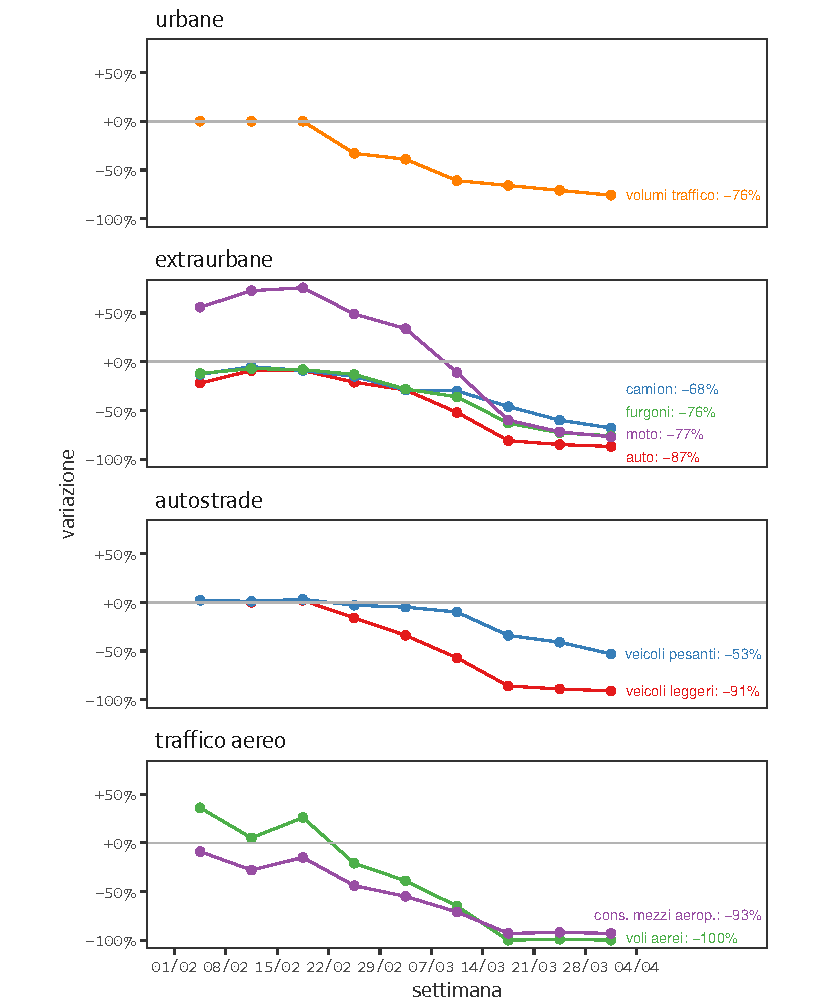
\includegraphics[width=\textwidth]{{figs/riduzioniDeterminanti_20200201-20200331}.pdf}
    \caption[Variazioni di indicatori relativi ad attività antropiche]{Variazioni settimanali di alcuni indicatori relativi ad attività antropiche rilevanti per la qualità dell'aria. Dall'alto: traffico su strade urbane, extra-urbane e autostrade; in fondo: traffico aereo.}
    \label{fig:riduzionedeterminanti}
\end{figure}

\FloatBarrier

\subsection{Contesto meteorologico}\label{cap:meteo}
L’analisi preliminare delle condizioni meteorologiche nel periodo oggetto di studio è di fondamentale importanza al fine di una corretta interpretazione degli effetti delle azioni di contenimento e della conseguente riduzione delle emissioni inquinanti sulla qualità dell'aria.

Per offrire una rappresentazione sintetica e qualitativa della capacità dell'atmosfera di disperdere e diluire gli inquinanti, o al contrario della tendenza ad accumularli, si sono calcolati tre indicatori:
    \begin{itemize}
        \item \textbf{stagnazione}: identifica condizioni persistenti di vento molto debole nello strato più basso; operativamente calcolata su base giornaliera come frazione delle 24 ore in cui $ws<ws_{crit}$, con $ws_{crit}=2~m/s$, velocità del vento critica oraria\citep{allwine1994single}
        \item \textbf{ricircolo}: identifica giornate caratterizzate da variabilità della direzione del vento, in particolare brezze; calcolata su base giornaliera: $$R=1-\frac{D_{net}}{D_{tot}}$$ con $D_{net}=\sqrt{\sum(u_i^2)+\sum(v_i^2)}$ e $D_{tot}=\sum(ws\cdot\Delta t)$ \citep{allwine1994single,perez2014atmospheric}
        \item \textbf{ventilazione}: identifica il ricambio della massa d'aria nello strato limite atmosferico; calcolata come media giornaliera della ventilazione oraria \citep{pasch2011meteorological,wu2013observational}
        $$V_h=\sum_{j=1}^{H_{ABL}}(dH_j \cdot ws_j)$$
    \end{itemize}

Le condizioni di bassa, media o alta criticità meteo sono valutate ogni giorno, per ciascuno dei tre indicatori, per le città di Trieste, Udine, Pordenone, Gorizia e Tolmezzo, in base alle soglie corrispondenti al 25\textsuperscript{o} e al 75\textsuperscript{o} percentile, calcolati sui dati 2016--2020 del trimestre febbraio--aprile.  

Si possono distinguere alcuni periodi (fig.\ref{fig:RSV}): 
\begin{description}
    \item [1 -- 5 febbraio] tre giornate favorevoli all'accumulo, specie a Tolmezzo, seguite da due giornate di maggiore ventilazione;
    \item [6 -- 26 febbraio] condizioni favorevoli all'accumulo a Tolmezzo e Udine, più favorevoli alla dispersione a Trieste, intermedie a Pordenone e Gorizia;
    \item [27 febbraio -- 7 marzo] condizioni favorevoli alla dispersione a Trieste e in parte anche a Gorizia, Pordenone e Udine;
    \item [8 -- 21 marzo] alternanza di giornale favorevoli alla dispersione e all'accumulo;
    \item [22 -- 31 marzo] condizioni decisamente favorevoli alla dispersione degli inquinanti, in tutta la regione;
    \item [1 -- 14 aprile] a Trieste prevalgono condizioni dispersive, mentre nel resto della regione si alternano a condizioni favorevoli all'accumulo;
    \item [15 -- 19 aprile] favorevoli all'accumulo a Trieste e Gorizia, intermedie altrove;
    \item [20 -- 30 aprile] tre giornate favorevoli alla dispersione, seguite da condizioni più intermedie.
\end{description}

In generale, a Trieste prevalgono condizioni di buona ventilazione, mentre Tolmezzo presenta condizioni meteo più critiche. Nella seconda metà del periodo in studio, su tutto il territorio regionale, l’atmosfera è in uno stato più favorevole alla dispersione (diminuzione) degli inquinanti. Dunque la dinamica dell'atmosfera potrebbe assumere un ruolo confondente nella ricerca degli effetti del \textit{lockdown}. Ciò richiederà particolare attenzione e analisi specifiche.

L'analisi dei giorni tipo della velocità del vento (fig.\ref{fig:giornivento}), calcolati ogni tre settimane come mediana per ciascuna delle 24 ore e confrontati con gli anni precedenti, conferma la maggiore ventosità nelle settimane 14 marzo -- 24 aprile, specie a Trieste, Udine e Gorizia\footnote{per la zona di Gorizia si considera la stazione di Capriva del Friuli}. Tuttavia le modulazioni del vento nell'arco della giornata, caratteristiche delle stazioni di Capriva, Tolmezzo e Udine, sono in linea con gli andamenti degli anni precedenti. Ciò aiuterà nell'interpretazione dei giorni tipo delle concentrazioni di inquinanti.

A fine marzo la configurazione meteorologica a grande scala ha determinato il trasporto in quota di notevoli masse di polveri di origine desertica dalle regioni vicine al Mar Caspio verso ovest. Tra il 27 e il 29 marzo hanno raggiunto anche il Friuli Venezia Giulia.

\begin{figure}
    \centering
    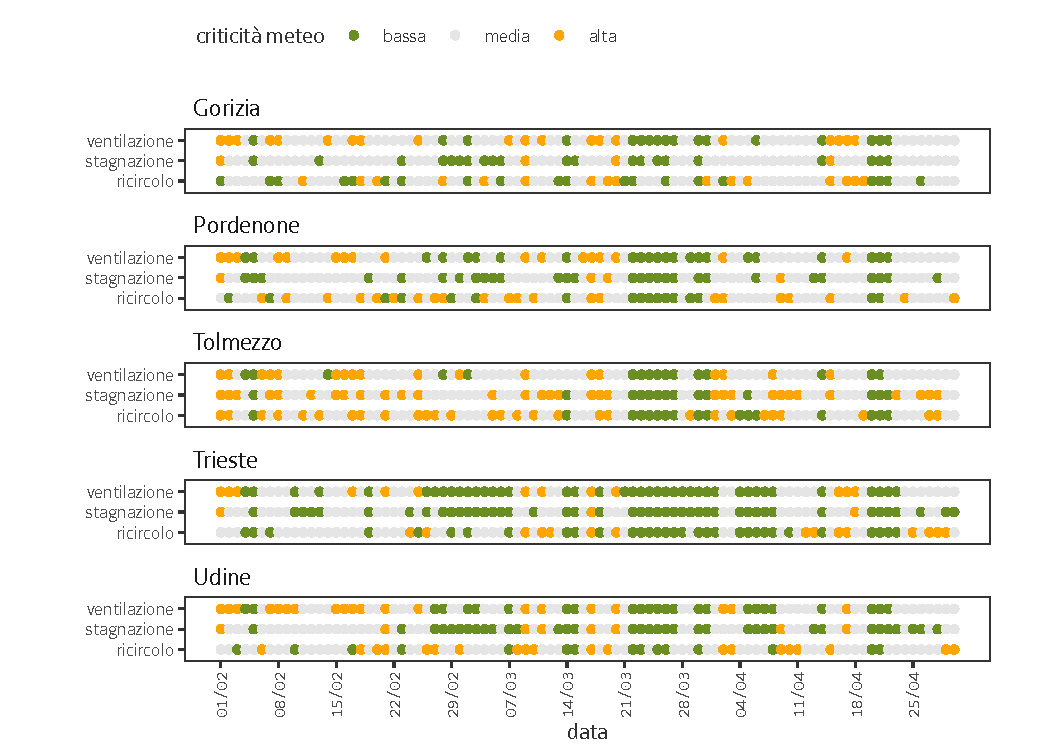
\includegraphics[width=\textwidth]{{figs/RecStaVen_20200201-20200430}.pdf}
    \caption[Indicatori meteo: ricircolo, stagnazione, ventilazione]{Indicatori meteorologici rilevanti per la qualità dell'aria (ricircolo, stagnazione, ventilazione) nel trimestre febbraio-aprile 2020}
    \label{fig:RSV}
\end{figure}

\begin{figure}
    \centering
    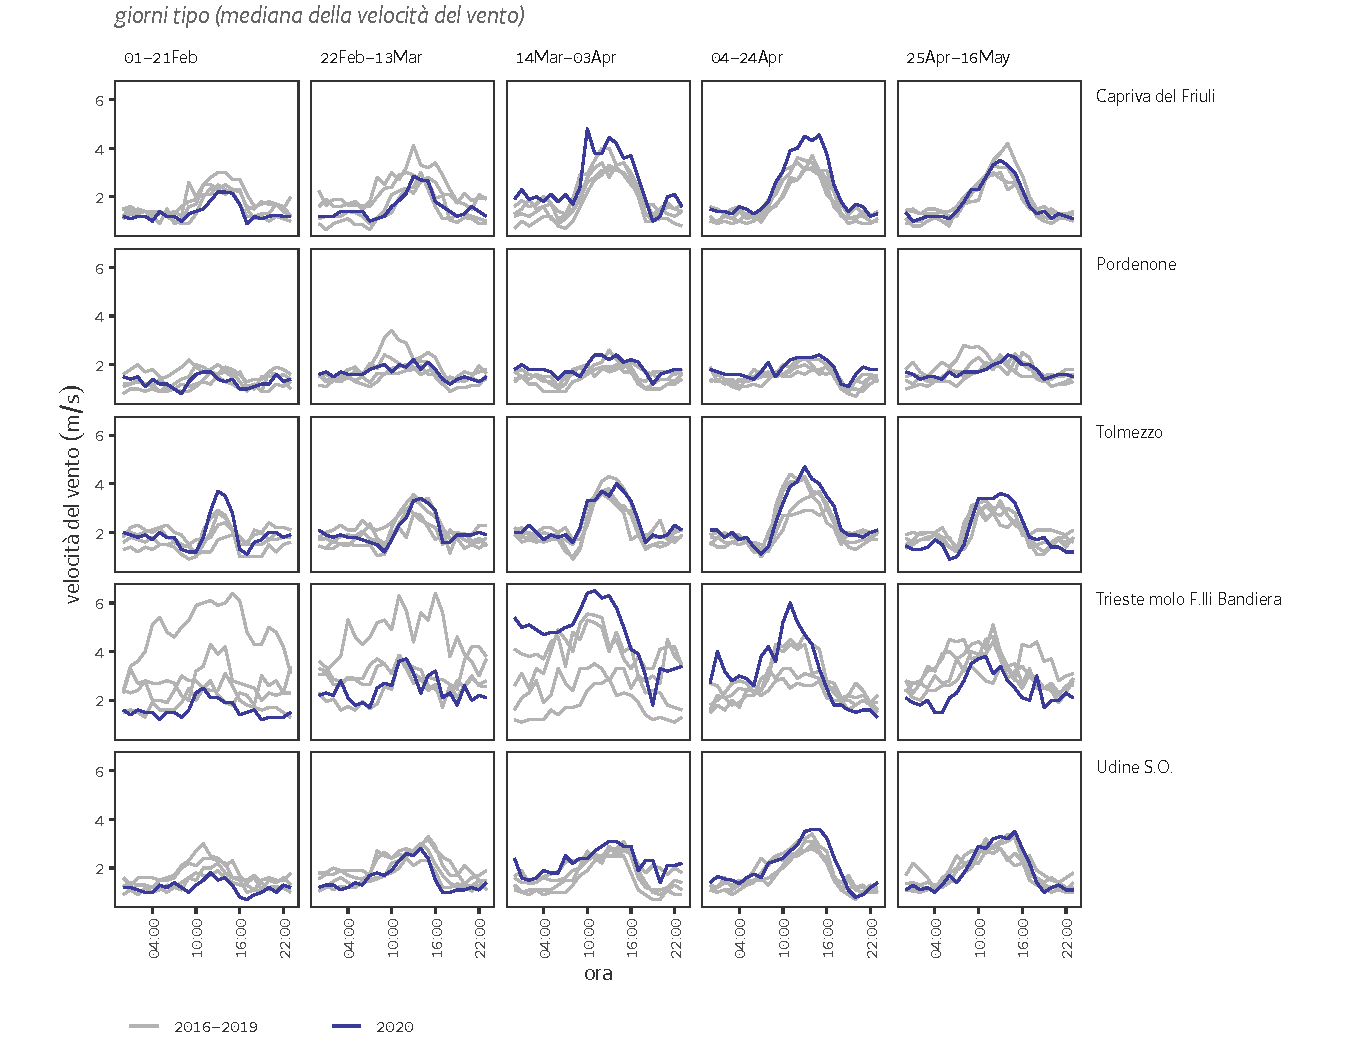
\includegraphics[width=\textwidth]{{figs/WindSpeed_MedianDay_LastVsPast_20200201-20200516}.pdf}
    \caption[Giorni tipo della velocità del vento]{Giorni tipo della velocità del vento, calcolati ogni tre settimane come mediana per ciascuna delle 24 ore. Confronto del 2020 con i 4 anni precedenti.}
    \label{fig:giornivento}
\end{figure}


\FloatBarrier
\section{Pressioni}\label{cap:pressioni}
\subsection{Emissioni in atmosfera}
A partire dalle variazioni di alcuni indicatori relativi al traffico su strada e al traffico aereo, registrate durante il periodo del \textit{lockdown} e descritte nella sezione precedente di questo \textit{report}, sono state stimate le corrispondenti variazioni delle emissioni di alcuni inquinanti in atmosfera.

La base dati di partenza è l'ultima versione disponibile dell'inventario delle emissioni del Friuli Venezia Giulia\footnote{\url{http://www.arpa.fvg.it/cms/tema/aria/pressioni/Catasto_emissioni/catasto.html}}, realizzato da ARPA-FVG con tecnologia INEMAR e riferito all'anno 2013. Dalla base dati sono state escluse alcune emissioni puntuali rilevanti, non attive durante il periodo di studio: la centrale termoelettrica di Monfalcone e l'area a caldo dell'impianto siderurgico di Servola (Trieste).

A partire dalle emissioni totali annuali, le emissioni settimanali in condizioni ``normali'' (cioè in assenza di azioni di contenimento del contagio) sono state calcolate con profili temporali standard.

Le variazioni settimanali degli indicatori di attività registrate nel 2020 sono state considerate rappresentative per tutto il territorio regionale. A partire da esse, le variazioni delle corrispondenti emissioni sono state calcolate con una proporzionalità lineare diretta. Per esempio, la diminuzione del 76\% nei conteggi di veicoli osservata l'ultima settimana di marzo a Pordenone è stata applicata alle emissioni per quella settimana di tutte le aree urbane della regione e di tutte le tipologie di veicoli, a prescindere dal carburante usato e dalla classe veicolare.

Si sono così stimate le variazioni, rispetto alle condizioni attese in assenza delle azioni di contenimento, delle emissioni antropiche regionali in atmosfera. Tali stime di variazione tengono dunque conto solo dei trasporti su strada e del traffico aereo, considerando invece invariate le attività produttive industriali e agricole, i traffici portuali, la produzione energetica e i consumi per il riscaldamento domestico. Tali variazioni potranno essere valutate nei prossimi mesi, quando ulteriori dati saranno disponibili.

L'analisi evidenzia (fig.\ref{fig:riduzioneemissioni}) un calo continuo nelle emissioni tra l'ultima settimana di febbraio e la fine di marzo 2020. Particolarmente marcato il calo delle emissioni di ossidi di azoto (NO\textsubscript{x}), che raggiunge il -25\%, dell'anidride carbonica (CO\textsubscript{2}, -19\%) e del monossido di carbonio (CO, -17\%). Meno netto il calo delle emissioni di polveri sottili (PM10 e PM2.5), inferiore al 10\% e probabilmente almeno in parte compensato dall'aumento nei consumi per riscaldamento domestico a biomassa\footnote{non stimato in questo \textit{report}}. Infine, le emissioni dei composti organici volatili nel loro insieme (COV), di ammoniaca (NH\textsubscript{3}) e di biossido di zolfo (SO\textsubscript{2}) non hanno subito variazioni di rilievo.

Nella prossima sezione si vedrà come a queste riduzioni emissive diversificate corrispondano, anche nelle concentrazioni misurate in aria, effetti differenziati per le varie specie chimiche monitorate.

\begin{figure}
    \centering
    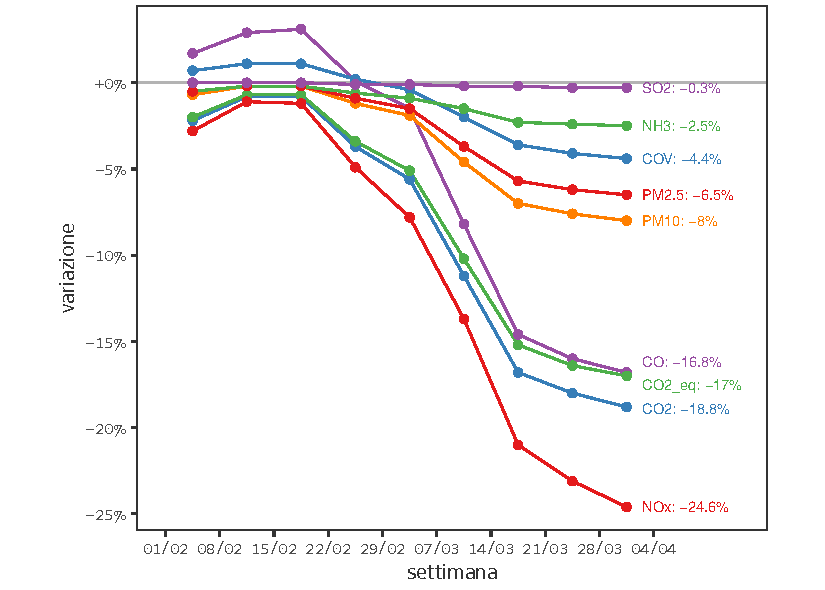
\includegraphics[width=\textwidth]{{figs/riduzioniEmissioni_20200201-20200331}.pdf}
    \caption[Riduzioni delle emissioni antropogeniche]{Riduzioni settimanali delle emissioni antropogeniche delle principali specie chimiche inquinanti e climalteranti in Friuli Venezia Giulia, stimate a partire dagli indicatori disponibili, riferiti al traffico stradale e aereo.}
    \label{fig:riduzioneemissioni}
\end{figure}


\FloatBarrier
\section{Stato}
\subsection{Qualità dell'aria: andamento}\label{cap:qaria}
Analizzando le concentrazioni misurate dalle stazioni di monitoraggio della qualità dell'aria e confrontandole con le misure degli anni precedenti, possiamo verificare se le riduzioni di emissioni (fig.\ref{fig:riduzioneemissioni}) abbiano determinato effetti sulla qualità dell'aria, e di quale entità. 

Gli andamenti delle mediane giornaliere regionali di benzene C\textsubscript{6}H\textsubscript{6}, biossido di azoto NO\textsubscript{2}, ozono O\textsubscript{3}, polveri sottili PM10 e PM2.5 (fig.\ref{fig:andaminq}), mostrano alcuni scostamenti del 2020 rispetto agli anni precedenti.

Il \textbf{benzene} ha generalmente concentrazioni più basse rispetto agli anni precedenti (fig.\ref{fig:andaminq}, primo pannello), ma poiché questa tendenza è già evidente prima del \textit{lockdown} e della chiusura delle scuole, è da attribuirsi ad una diminuzione delle emissioni che prescinde dalle azioni di contenimento. Tale tendenza si nota anche nell'analisi dei giorni tipo di alcune stazioni di monitoraggio, per esempio CAI (Udine, fig.\ref{fig:giornibenzene}). Inoltre, le stazioni industriali di Trieste (PIT e PON, fig.\ref{fig:giornibenzene}) non hanno registrato i picchi osservati negli anni scorsi, ascrivibili alle emissioni dell'area a caldo del polo siderurgico, ormai inattiva.

Il \textbf{biossido di azoto}, NO\textsubscript{2}, ha concentrazioni in linea con gli anni precedenti nelle prime settimane di febbraio (fig.\ref{fig:andaminq}, secondo pannello). Il calo progressivo che si osserva nei giorni 27 febbraio -- 7 marzo potrebbe essere determinato sia dalla chiusura delle scuole sia dalle condizioni meteo favorevoli alla dispersione (cfr.fig.\ref{fig:RSV}). Invece l'ulteriore calo nel periodo successivo, seppur accompagnato da fluttuazioni coerenti con le condizioni meteo, è da attribuire agli effetti del \textit{lockdown}. Infatti esso interessa tutta la regione (fig.\ref{fig:giornino2}, terza e quarta colonna) e corrisponde a un netto smorzamento dei picchi corrispondenti alle ore di punta nel traffico stradale, la mattina e la sera.

L'\textbf{ozono}, inquinante secondario di origine fotochimica, non risente in maniera evidente degli effetti del \textit{lockdown}. Le concentrazioni di aprile, più alte degli anni precedenti (fig.\ref{fig:andaminq}, terzo pannello), sono da attribuirsi alle temperature particolarmente miti di quelle settimane. I giorni medi conservano l'andamento tipico (fig.\ref{fig:giornio3}).

Le polveri \textbf{PM10} mostrano un vistoso picco di concentrazioni corrispondenti al trasporto a grande scala di polveri di origine desertica che ha interessato il Friuli Venezia Giulia nei giorni 27-29 marzo (fig.\ref{fig:andaminq}, quarto pannello). Il picco è meno marcato per le polveri più sottili \textbf{PM2.5} (fig.\ref{fig:andaminq}, quinto pannello), segno che le polveri desertiche avevano una granulometria grossolana. Al di là di questo fattore confondente, non si notano particolari scostamenti rispetto agli anni precedenti, neppure nei giorni tipo (fig.\ref{fig:giornipm10}). Si rimanda perciò all'analisi sulla granulometria delle polveri (pag.\ref{cap:cef} e sgg.).


\begin{figure}
    \centering
    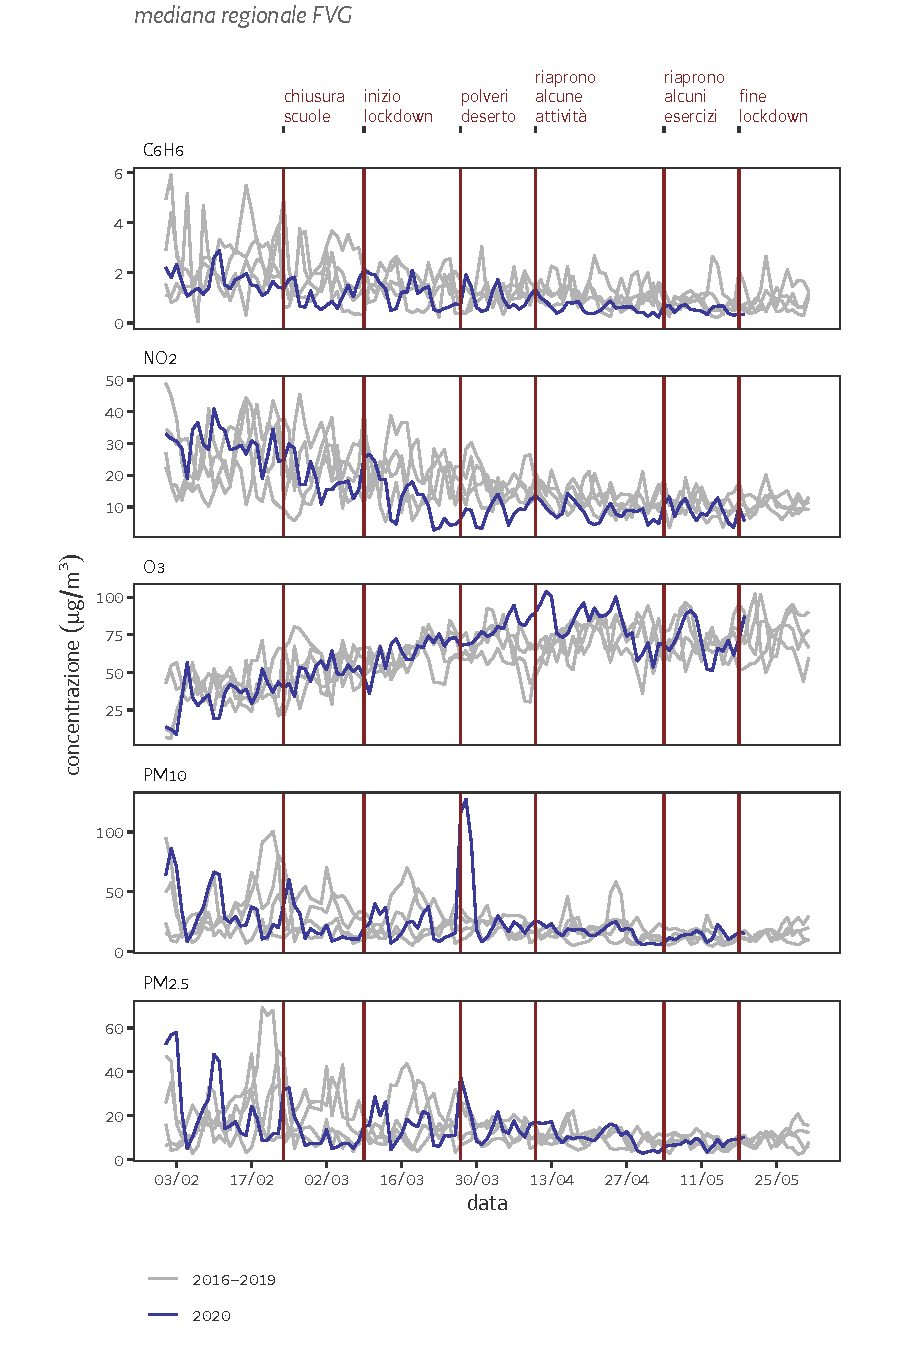
\includegraphics[trim=0 0 0 1cm, clip,width=0.85\textwidth]{{figs/dailyLastVsPast_20200201-20200531}.pdf}
    \caption[Andamento delle concentrazioni dei principali inquinanti, mediana regionale]{Andamento delle concentrazioni aria ambiente dei principali inquinanti, nel periodo febbraio--maggio 2020. Mediane giornaliere regionali in Friuli Venezia Giulia, confrontate con lo stesso periodo degli anni precedenti. Dall'alto: benzene, biossido di azoto, ozono, polveri sottili PM10 e PM2.5}
    \label{fig:andaminq}
\end{figure}

\begin{figure}
    \centering
    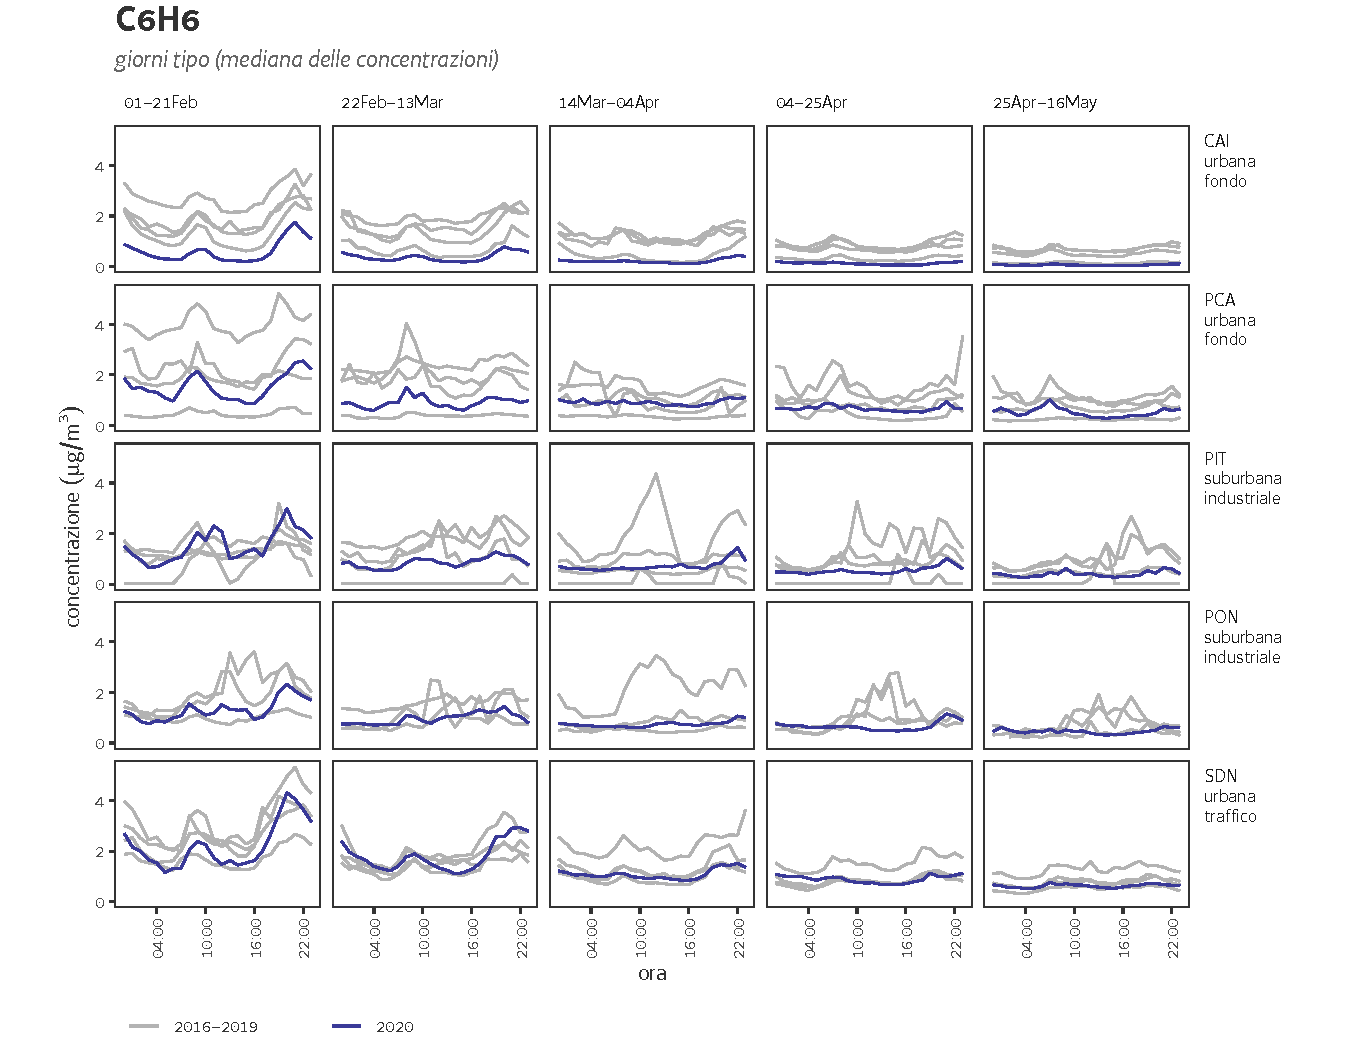
\includegraphics[width=\textwidth,page=1]{{figs/medianDay_LastVsPast_20200201-20200516}.pdf}
    \caption[Giorni tipo del benzene]{Giorni tipo delle concentrazioni di benzene calcolati ogni tre settimane nel periodo 1 febbraio -- 16 maggio 2020, confrontati con gli anni precedenti.}
    \label{fig:giornibenzene}
\end{figure}

\begin{figure}
    \centering
    \includegraphics[width=\textwidth,page=2]{{figs/medianDay_LastVsPast_20200201-20200516}.pdf}
    \caption[Giorni tipo del biossido di azoto]{Giorni tipo delle concentrazioni di biossido di azoto calcolati ogni tre settimane nel periodo 1 febbraio -- 16 maggio 2020, confrontati con gli anni precedenti.}
    \label{fig:giornino2}
\end{figure}

\begin{figure}
    \centering
    \includegraphics[width=\textwidth,page=3]{{figs/medianDay_LastVsPast_20200201-20200516}.pdf}
    \caption[Giorni tipo dell'ozono]{Giorni tipo delle concentrazioni di ozono calcolati ogni tre settimane nel periodo 1 febbraio -- 16 maggio 2020, confrontati con gli anni precedenti.}
    \label{fig:giornio3}
\end{figure}

\begin{figure}
    \centering
    \includegraphics[width=\textwidth,page=4]{{figs/medianDay_LastVsPast_20200201-20200516}.pdf}
    \caption[Giorni tipo del PM10]{Giorni tipo delle concentrazioni di polveri sottili PM10 calcolati ogni tre settimane nel periodo 1 febbraio -- 16 maggio 2020, confrontati con gli anni precedenti.}
    \label{fig:giornipm10}
\end{figure}

\FloatBarrier
%\subsection{Qualità dell'aria: test statistici}
\subsection{Rapporti tra inquinanti}\label{cap:rapporti}
Come si è detto nella sezione dedicata al contesto meteo (par.\ref{cap:meteo}, pag.\pageref{cap:meteo} e sgg.), l'aumento della ventilazione verificatosi in corrispondenza dell'entrata in vigore delle misure di distanziamento e di limitazione della mobilità può costituire un elemento confondente nell'individuazione degli effetti sulla qualità dell'aria del \textit{lockdown}. 

Un modo per aggirare questa interferenza è analizzare i rapporti tra concentrazioni di inquinanti. Infatti i fattori meteo che determinano dispersione degli inquinanti, quali la turbolenza e la ventosità, e quelli che ne determinano l'accumulo agiscono per lo più in maniera ``aspecifica'', cioè senza distinguere tra inquinanti. 
Perciò in prima approssimazione ci si può aspettare che il rapporto tra le concentrazioni di alcuni inquinanti resti sostanzialmente inalterato a prescindere dalla meteorologia.
Dunque l'analisi dei rapporti tra concentrazioni di inquinanti consente di ridurre l'effetto confondente della meteorologia, focalizzandosi meglio sugli effetti delle variazioni delle emissioni.

\FloatBarrier\paragraph{Toluene/benzene}\label{cap:tb}
Il rapporto tra le concentrazioni dei composti organici toluene e benzene è comunemente utilizzato come indicatore della prossimità ad alcune sorgenti emissive. In generale, le emissioni da traffico veicolare, attività industriali e uso di solventi determinano valori del rapporto toluene/benzene superiori ad 1, mentre le emissioni da combustione di biomassa, biocombustibili e carbone determinano valori inferiori a 1 \cite{zhang2016spatiotemporal,seco2013volatile}. 

Dunque l'analisi di questo rapporto prima e durante l'attuazione delle azioni di limitazione alla mobilità individuale, e in particolare il confronto con gli anni precedenti e tra stazioni collocate a distanze diverse dalle strade, può consentire di individuare gli effetti del \textit{lockdown} sulle concentrazioni di composti organici in aria ambiente.

Prima dell'entrata in vigore delle misure di contenimento il rapporto toluene/benzene presentava valori generalmente compresi tra 1 e 2, mentre durante il \textit{lockdown} tale rapporto, pur con alcune fluttuazioni, ha spesso raggiunto valori di 0.5 o anche inferiori (fig.\ref{fig:tbandamento}). Questa evidente variazione può essere in parte attribuita alla netta diminuzione dei flussi di traffico veicolare, in parte ad un probabile lieve aumento delle emissioni da combustione di biomassa per riscaldamento domestico. Temporanei aumenti del consumo di legna per il riscaldamento domestico sono probabilmente la causa delle analoghe diminuzioni del rapporto toluene/benzene osservate occasionalmente negli anni precedenti, durante settimane caratterizzate da temperature particolarmente rigide.

La figura \ref{fig:tbgiorni} riporta i giorni tipo del rapporto toluene/benzene calcolati su periodi di tre settimane ciascuno. Questa suddivisione consente di analizzare separatamente periodi abbastanza omogenei per condizioni meteorologiche e per grado di applicazione delle misure di contenimento del contagio. I grafici della prima colonna riportano l’andamento del giorno tipo prima del \textit{lockdown}, la seconda si riferisce al periodo di sola chiusura delle scuole, le successive due colonne riportano gli andamenti durante il blocco, mentre l’ultima è riferita al periodo in cui il blocco viene parzialmente allentato.

Considerando in particolare le stazioni di Udine (CAI e SDN, fig.\ref{fig:tbgiorni}) si osservano, tanto nel terzo quanto nel quarto periodo, apprezzabili differenze con gli anni precedenti. In particolare, nel terzo periodo (14 marzo -- 04 aprile) il rapporto toluene/benzene risulta essere significativamente inferiore rispetto al quadriennio 2016--2019 durante tutto l’arco della giornata. Nel quarto periodo, caratterizzato da una ventilazione che nel complesso risulta comparabile a quella del quinquennio precedente, il rapporto toluene/benzene evidenzia una apprezzabile diminuzione nelle sole ore pomeridiane; il fenomeno può essere spiegato con l’aumento dei livelli di ozono che è stato registrato in quel periodo e alla conseguente diminuzione delle concentrazioni di toluene nell’aria (che viene rimosso tramite reazioni di degradazione ossidativa).
Nel  quinto e ultimo periodo (nel quale lentamente riprendono alcune attività produttive) i giorni tipo si riallineano con gli anni scorsi.


\begin{figure}
    \centering
    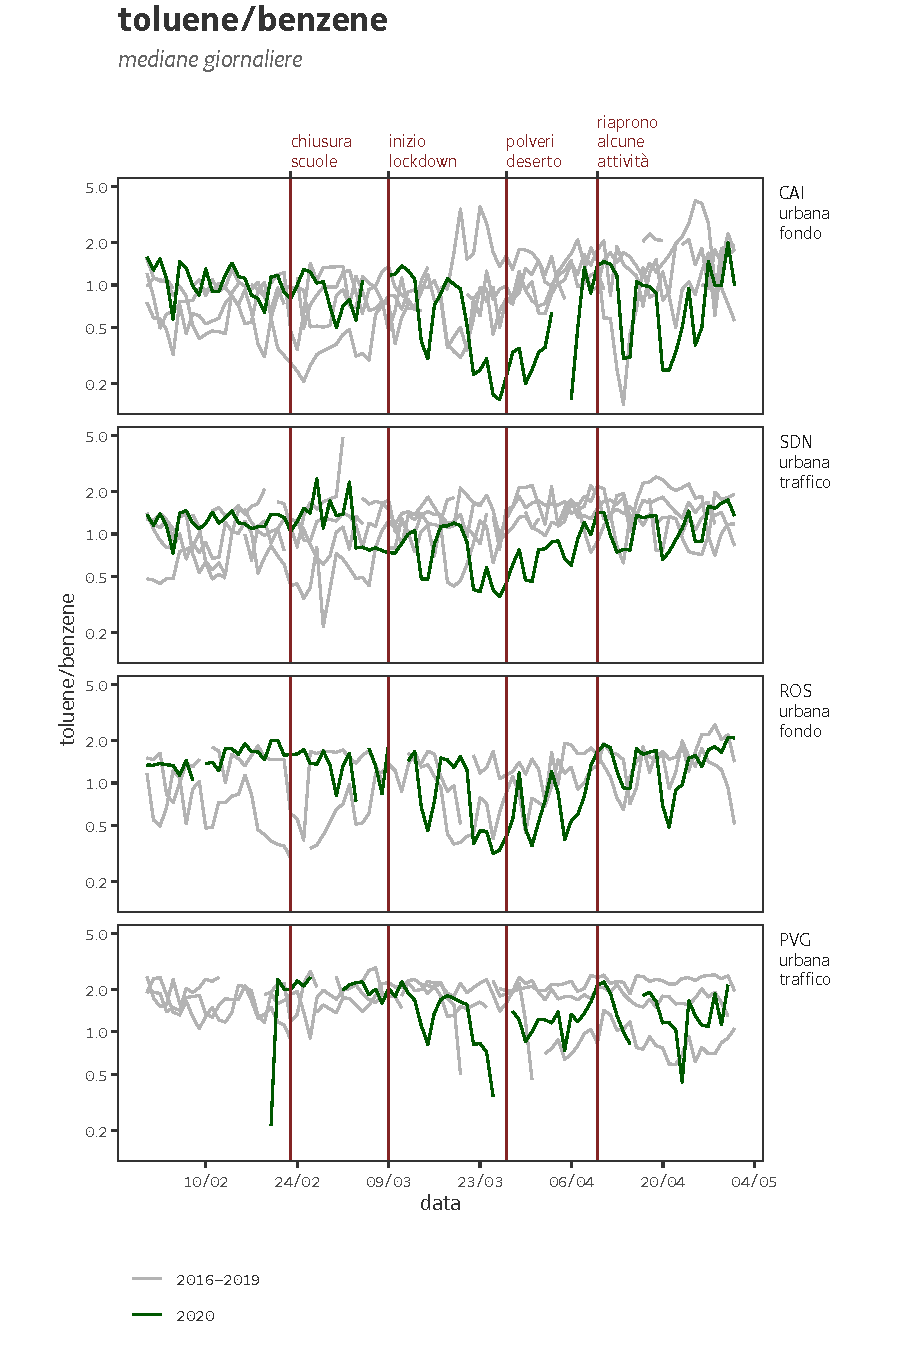
\includegraphics[trim=0 0 0 2cm, clip, width=0.9\textwidth]{{figs/dailyLastVsPast_TB_20200201-20200501}.pdf}
    \caption[Andamento del rapporto toluene/benzene]{Andamento del rapporto toluene/benzene nel periodo febbraio--aprile 2020. Mediane giornaliere confrontate con gli anni precedenti.}
    \label{fig:tbandamento}
\end{figure}

\begin{figure}
    \centering
    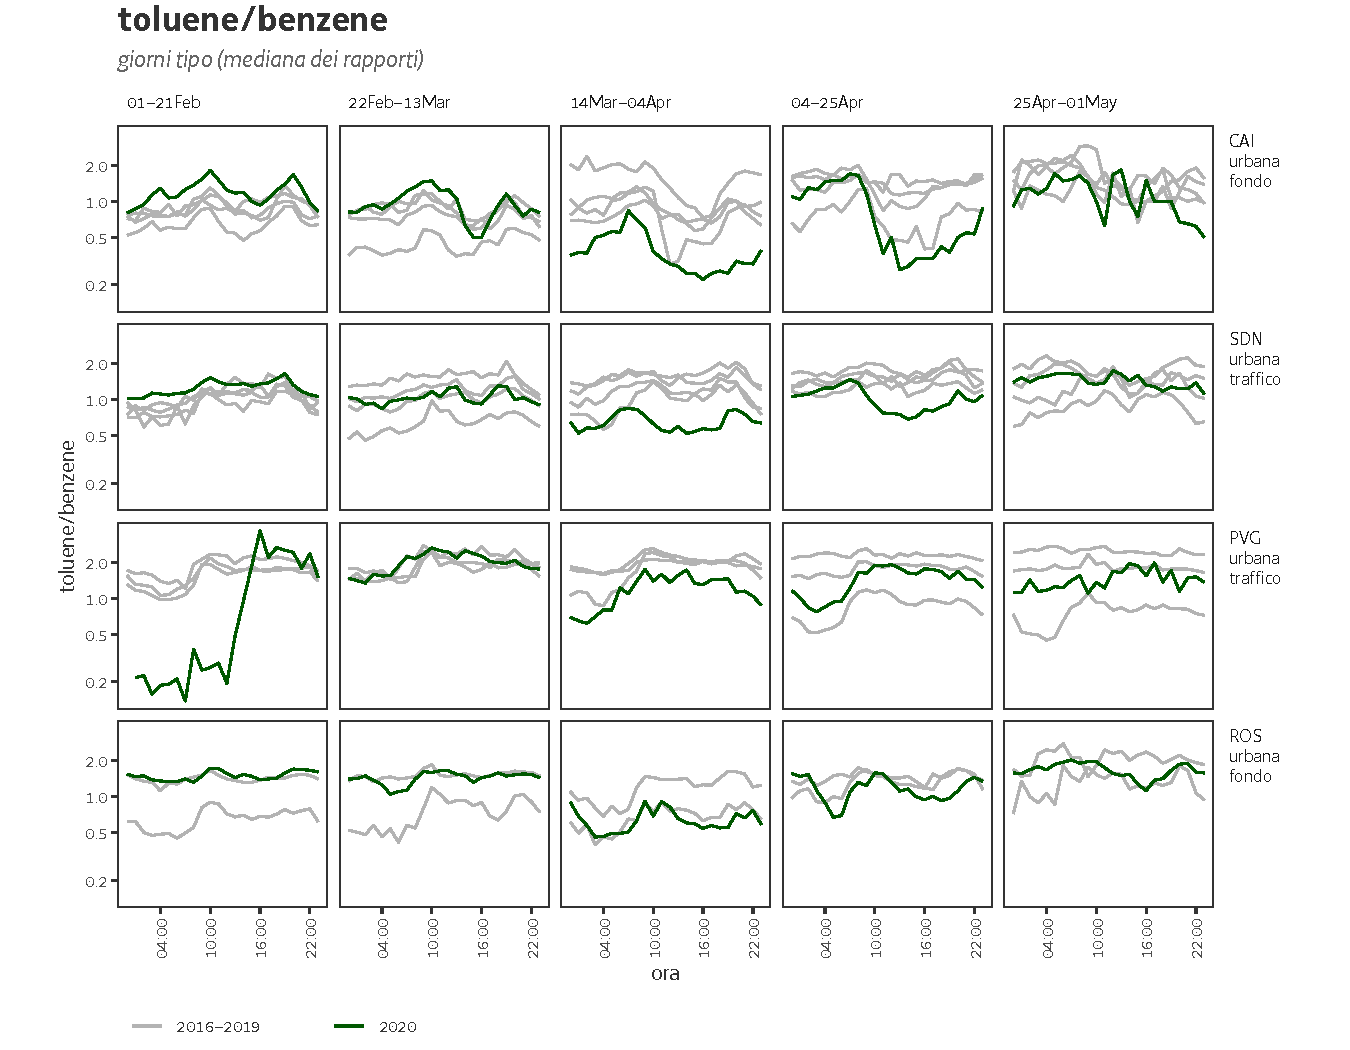
\includegraphics[width=\textwidth]{{figs/medianDay_LastVsPast_TB_20200201-20200501}.pdf}
    \caption[Giorni tipo del rapporto toluene/benzene]{Giorni tipo del rapporto toluene/benzene calcolati ogni tre settimane nel periodo febbraio--aprile 2020, confrontati con gli anni precedenti.}
    \label{fig:tbgiorni}
\end{figure}

%\begin{figure}
%    \centering
%    \includegraphics[width=0.9\textwidth]{{figs/daily_TB_20200201-2020043%0}.pdf}
%    \caption[Rapporto toluene/benzene, confronto tra stazioni]{Andamento del rapporto toluene/benzene nel periodo febbraio--aprile 2020. Mediane giornaliere, confronti tra stazioni della stessa città.}
%    \label{fig:tbconfronti}
%\end{figure}

\FloatBarrier
\paragraph{Ossidi di azoto}\label{cap:noxno}

Fermo restando il ruolo delle condizioni meteo nell’azione di dispersione degli inquinanti atmosferici, il rapporto diagnostico NOx/NO è una grandezza adimensionale il cui valore dipende sia dalla distanza delle fonti emissive di ossidi di azoto sia dai fattori che influenzano la   cinetica chimica dell’ossidazione dell’NO a NOx durante il corso della giornata.

Essendo la specie NO un inquinante primario emesso direttamente dal traffico veicolare, il rapporto NOx/NO viene indagato per poter comprendere se vi siano variazioni peculiari durante il periodo di \textit{lockdown} rispetto agli andamenti degli anni precedenti, considerando sia stazioni da traffico direttamente interessate dal blocco veicolare sia stazioni di fondo per confronto.
In seguito al blocco infatti il flusso di traffico è diminuito drasticamente in regione (fig.\ref{fig:riduzionedeterminanti}) pertanto ci si attende che la riduzione di una fonte importante di NO provochi un aumento contestuale del rapporto diagnostico NOx/NO.

La figura \ref{fig:noxandamento} riporta l’andamento del valore mediano giornaliero del rapporto NOx/NO riferito al periodo febbraio -- aprile 2020 (linea verde) confrontato con i trend misurati per il medesimo periodo negli ultimi 5 anni di monitoraggio (linee grigie).
Osserviamo che le stazioni più suscettibili all’aumento del rapporto NOx/NO sembrano essere quelle da traffico (SDN a Udine, AOS a Gorizia e soprattutto PNC a Pordenone) in cui il blocco ha ridotto sensibilmente le concentrazioni di NO con conseguente aumento  del rapporto diagnostico. Per la stazione da traffico PVG di Trieste il trend è meno evidente.
Le stazioni di fondo (CAI e ROS) mostrano invece un andamento in linea con gli anni precedenti, segno che la riduzione delle emissioni dovuta al \textit{lockdown} ha avuto effetti più marcati in prossimità delle strade.

La figura \ref{fig:noxgiorni} riporta i giorni tipo del rapporto NOx/NO calcolati su periodi di tre settimane ciascuno. Questa suddivisione consente di analizzare separatamente periodi abbastanza omogenei per condizioni meteorologiche e per grado di applicazione delle misure di contenimento del contagio. I grafici della prima colonna riportano l’andamento del giorno tipo prima del \textit{lockdown}, la seconda si riferisce al periodo di sola chiusura delle scuole, le successive due colonne riportano gli andamenti durante il blocco, mentre l’ultima è riferita al periodo in cui il blocco viene parzialmente allentato.

In condizioni normali (prima colonna in fig.\ref{fig:noxgiorni}) il rapporto NOx/NO presenta i valori minimi in corrispondenza dei picchi di traffico, la mattina e la sera, e i valori massimi nelle ore notturne, quando quasi tutto l’NO prodotto nella fase diurna viene ossidato a NOx. Con l'attuazione del blocco (terza e quarta colonna) viene meno il minimo serale e in generale i valori del rapporto NOx/NO aumentano, in alcune stazioni di traffico (Pordenone 14 marzo -- 25 aprile, Gorizia 25 aprile -- 1 maggio) discostandosi dagli andamenti degli anni precedenti. Tuttavia lo scostamento dei giorni medi di NOx/NO rientra nella maggior parte dei casi nell'intervallo di naturale variabilità interannuale.

\begin{figure}
    \centering
    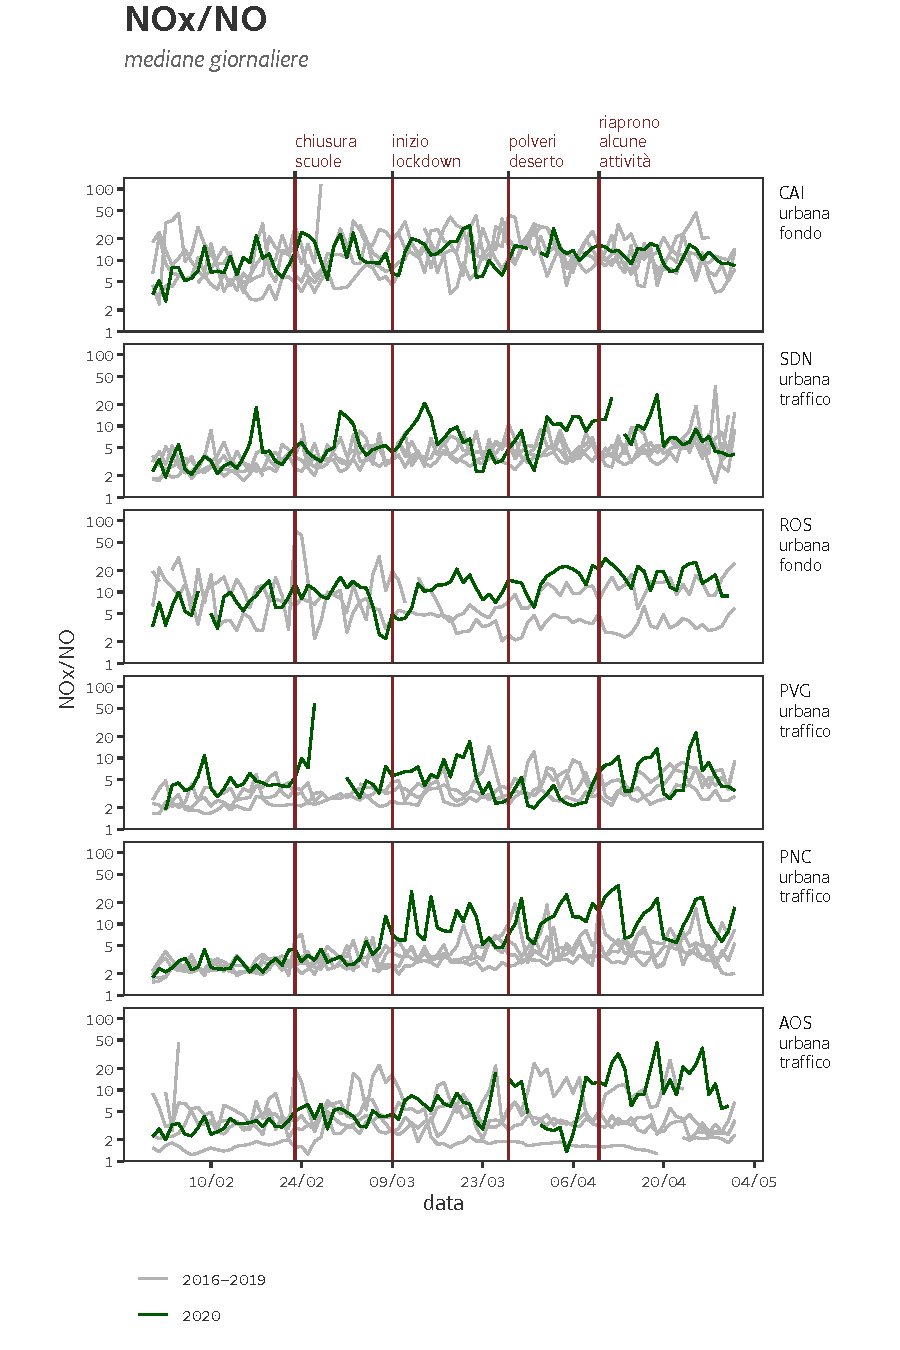
\includegraphics[trim=0 0 0 2cm, clip,width=0.9\textwidth]{{figs/dailyLastVsPast_NOXNO_20200201-20200501}.pdf}
    \caption[Andamento del rapporto NOx/NO]{Andamento del rapporto NOx/NO nel periodo febbraio--aprile 2020. Mediane giornaliere confrontate con gli anni precedenti.}
    \label{fig:noxandamento}
\end{figure}

\begin{figure}
    \centering
    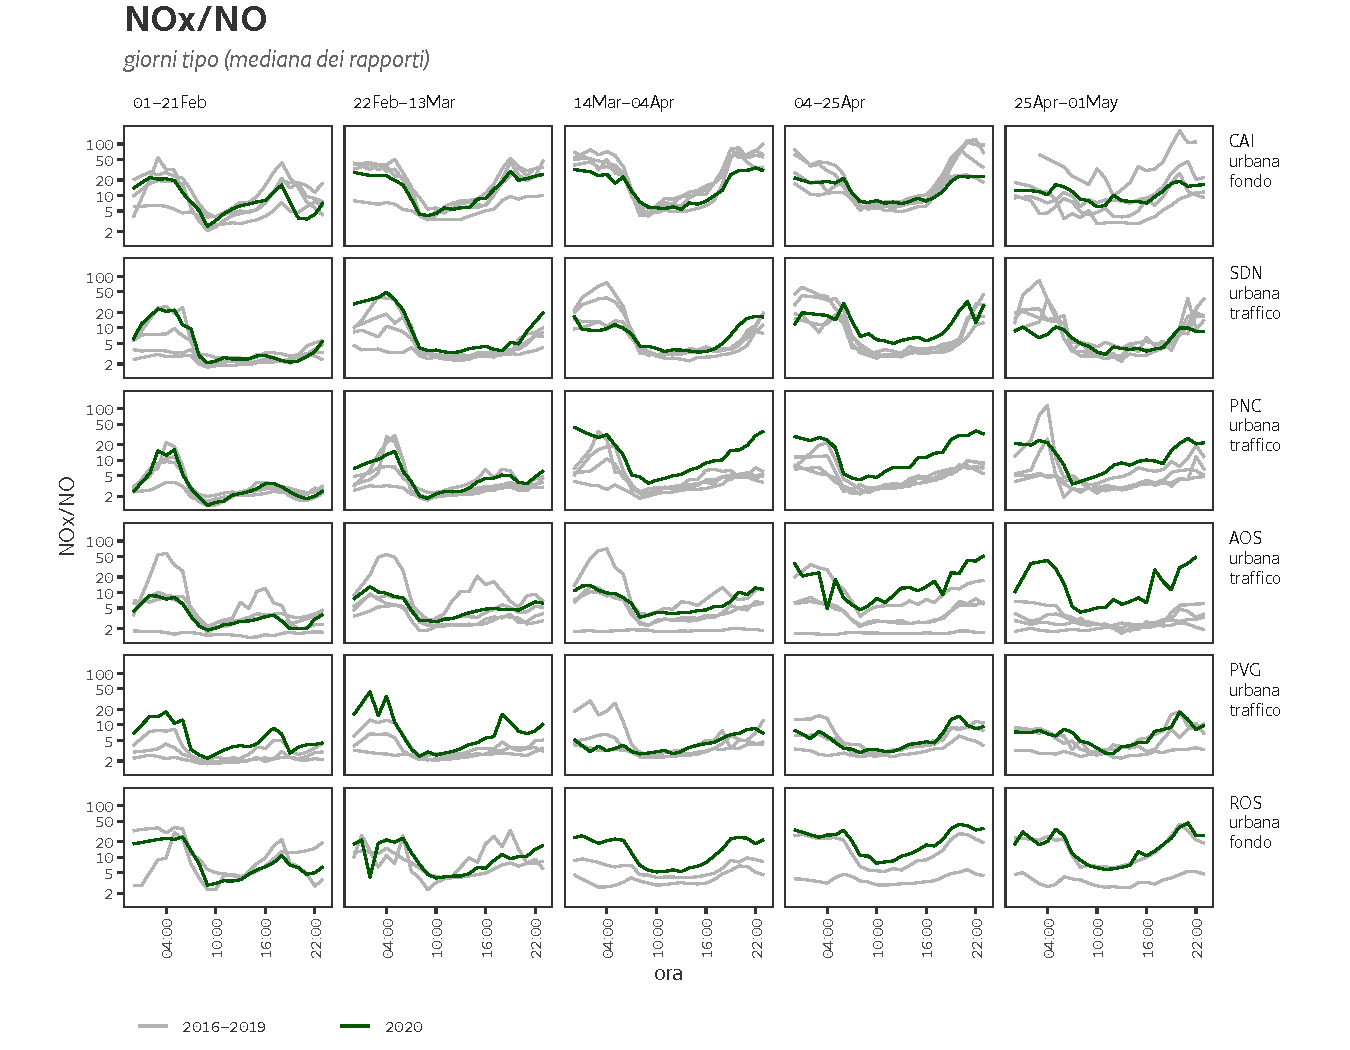
\includegraphics[width=\textwidth]{{figs/medianDay_LastVsPast_NOXNO_20200201-20200501}.pdf}
    \caption[Giorni tipo del rapporto NOx/NO]{Giorni tipo del rapporto NOx/NO calcolati ogni tre settimane nel periodo febbraio--aprile 2020, confrontati con gli anni precedenti.}
    \label{fig:noxgiorni}
\end{figure}

%\begin{figure}
%    \centering
%    \includegraphics[width=0.9\textwidth]{{figs/daily_NOXNO_20200201-2020%0430}.pdf}
%    \caption[Rapporto NOx/NO, confronto tra stazioni]{Andamento del rapporto NOx/NO nel periodo febbraio--aprile 2020. Mediane giornaliere, confronti tra stazioni della stessa città.}
%    \label{fig:noxconfronti}
%\end{figure}

\FloatBarrier
\paragraph{Granulometria delle polveri}\label{cap:cef}

Le frazioni granulometriche usualmente utilizzate per lo studio della formazione del materiale particolato (polveri) in atmosfera sono il PM\textsubscript{10} (polveri con diametro aerodinamico inferiore ai 10~micron), il  PM\textsubscript{2.5} (polveri con diametro aerodinamico inferiore ai 2.5~micron) e il  PM\textsubscript{coarse} ($PM_{10}-PM_{2.5}$, polveri con diametro aerodinamico compreso tra i 2.5 e i 10~micron).

Qui consideriamo il coefficiente di arricchimento percentuale della frazione \textit{coarse} (CEF, \textit{Coarse Enrichment Factor}) 
$$CEF=\frac{(PM_{10}-PM_{2.5})}{PM_{10}} \cdot 100$$

Questo parametro è adimensionale e variabile tra 0 e 100. Esso consente di valutare se l'andamento della frazione grossolana (\textit{coarse}) delle polveri sia correlato alle condizioni meteorologiche e/o alle sorgenti emissive locali.
 Per poter capire meglio gli andamenti e le dinamiche che governano questa grandezza è necessario sempre considerare almeno due punti di misura interessati da sorgenti emissive significativamente diverse (per esempio una stazione di fondo urbano e una stazione da traffico) ma anche spazialmente vicini e dunque soggetti alle stesse condizioni meteo. Così facendo le variabili meteo-climatiche che agiscono sulle due stazioni non rischiano di divenire un fattore confondente per la comprensione degli andamenti del CEF.  
Lo studio in oggetto ha riguardato siti di misura distanti pochi chilometri:  la stazione di Pordenone centro (urbana da traffico) e la stazione di Brugnera (suburbana di fondo).

Il periodo di misura considerato va dal 24/01 al 22/05/2020 comprendente pertanto una fase precedente al \textit{lockdown}, il \textit{lockdown} stesso e una fase successiva al blocco.
Dall'insieme di dati analizzati sono stati esclusi i giorni 27--29 marzo perché disturbati da episodi di ricaduta  di polveri grossolane provenienti dai deserti asiatici.
Inoltre dall'analisi sono escluse le giornate con $PM_{2.5}<7 \mu g/m^3$, cioè con concentrazioni di polveri molto basse.

La figura \ref{fig:cef} riporta gli andamenti medi giornalieri del CEF relativi alla stazione di traffico (Pordenone centro)  e la stazione di fondo suburbano (Brugnera) nel periodo considerato. Entrambe le stazioni sono situate nell'area pordenonese, perciò si possono considerare interessate, in prima approssimazione, dai medesimi determinanti meteo-climatici. 

Si nota un progressivo aumento del CEF nel corso del periodo, in parte attribuibile al graduale venir meno di una rilevante fonte emissiva di particolato fine, la combustione di legna negli impianti di riscaldamento domestici.

Ciò che è interessante rilevare è lo scarto tra la stazione di traffico e la stazione di fondo. Prima del blocco in prossimità delle strade si registra un CEF sistematicamente più alto, cioè un maggior contributo della frazione grossolana, probabilmente determinato dall'azione di risollevamento delle polveri depositate sull'asfalto, causata dal frequente passaggio di veicoli. Durante il \textit{lockdown} invece il CEF nelle due stazioni è molto simile, segno che è venuto meno quel contributo alla concentrazione di polveri sottili, importante ma limitato alle aree più urbanizzate e trafficate.

\begin{figure}
    \centering
    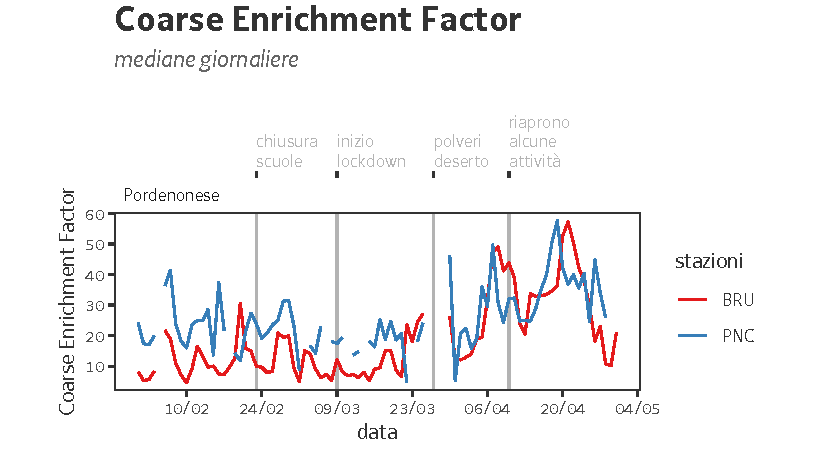
\includegraphics[trim=0 0 0 2cm, clip,width=0.9\textwidth]{{figs/daily_CEF_20200201-20200430}.pdf}
    \caption[Percentuale di polveri grossolane nel PM10, confronto tra stazioni]{Andamento della percentuale di polveri grossolane nel PM10 nel periodo febbraio--aprile 2020. Medie giornaliere, confronti tra stazioni dell'area pordenonese.}
    \label{fig:cef}
\end{figure}

\FloatBarrier
\subsection{Caratterizzazione chimica delle polveri sottili}\label{cap:chimica}
\paragraph{Metalli}\label{cap:metalli}
È noto dalla letteratura scientifica che alcuni metalli aerodispersi sono più strettamente legati al traffico veicolare, rispetto ad altri metalli che invece possono avere varie origini tra cui quella terrigena. In particolare antimonio Sb e rame Cu derivano dall’usura dei freni e dei contatti elettrici, \cite{iijima2008emission,iijima2009clarification}.  Per questo motivo, per l’indagine sul \textit{lockdown}, si è scelto di valutare anche l’andamento delle concentrazioni dei metalli in aria ambiente.

In regione, l’unica stazione di fondo urbano utilizzata per il monitoraggio delle concentrazioni dei metalli rimane, ad oggi, la stazione di via Cairoli (Udine). Negli ultimi anni, infatti, le concentrazioni in aria ambiente dei metalli normati (arsenico As, cadmio Cd, nichel Ni, piombo Pb) sono sempre risultate molto al di sotto della soglia di valutazione inferiore e quindi, secondo norma, non è nemmeno necessario il loro monitoraggio; inoltre, studi chemiometrici\footnote{studi chemiometrici di modellamento di classe, SIMCA, condotti in collaborazione con l’Università La Sapienza di Roma} hanno verificato che il profilo di composizione chimica del PM10 delle principali stazioni urbane della Regione è, per quanto riguarda i metalli, lo stesso in tutte le città analizzate.

Per il presente studio sono stati quindi elaborati i dati di via Cairoli di marzo 2020 che sono stati anche confrontati coi dati dei due anni precedenti, raccolti nello stesso periodo. Fra tutti i metalli analizzati si è deciso di trattare solamente quelli ben determinabili dal punto di vista analitico (almeno metà dei dati quantificabile) e/o che denotassero delle correlazioni evidenti nella matrice di correlazione (qui non riportata). I metalli selezionati sono stati antimonio Sb e rame Cu (fra loro ben correlati e indicativi del traffico veicolare) nonché ferro Fe, manganese Mn e piombo Pb (fra loro ben correlati e a loro volta ben correlati col PM10).

Le concentrazioni medie in aria ambiente calcolate nel periodo pre-\textit{lockdown} (2-12 marzo 2020, 6 campioni) e nel periodo di \textit{lockdown} (14-26 marzo 2020, 6 campioni) sono riportate in tabella \ref{tab:metalli}. Come si può osservare nell’ultima colonna della tabella, la diminuzione percentuale più drastica si è riscontrata proprio per Sb e Cu.

In figura \ref{fig:metalli1} si osserva il trend nel mese di marzo 2020 per quanto riguarda Sb e Cu (grafico in alto sinistra) e Fe, Mn, Pb e PM10 (grafico in alto a destra). Le concentrazioni sono state “riscalate” per singolo parametro (concentrazione n-esima / concentrazione massima) così da poter apprezzare simultaneamente gli andamenti di tutti i parametri. Come si può osservare, Sb e Cu presentano un andamento decrescente dall’inizio del mese in poi che non si osserva per gli altri metalli, che invece procedono all’unisono con le concentrazioni di PM10 (nei giorni 27-28-29 marzo si è avuto il fenomeno delle sabbie desertiche molto ben evidente nel grafico di destra). I picchi maggiori in entrambi i grafici, si verificano in concomitanza delle maggiori concentrazioni di polvere ma il trend è comunque diverso nei due casi. 

Sempre in figura \ref{fig:metalli1} si osserva invece che nel 2018 (grafico in basso a sinistra) e nel 2019 (in basso a destra) antimonio e rame presentano un trend confrontabile con quello degli altri metalli.

Al fine di catturare le variazioni della composizione del PM10 pre- e post-\textit{lockdown} tenendo in considerazione contemporaneamente tutti  i metalli analizzati, è stata condotta un’Analisi delle Componenti Principali (PCA). Si ottiene il \textit{biplot} (varianza spiegata: 94\%, di cui 63\% sulla PC1 e 31\% sulla PC2) presentato nella figura \ref{fig:metalli2}.

Emerge un’ottima separazione dei campioni di tipo “\textit{dust}” (polveri desertiche, contrassegnati con le “X” marroni, e situate a destra nel piano) da quelli di tipo urbano (a sinistra); tra questi ultimi, si nota una certa tendenza dei campioni pre-\textit{lockdown} (pallini viola) a localizzarsi nella parte alta del piano, mentre i campioni relativi al periodo di \textit{lockdown} (cerchietti azzurri) si localizzano mediamente più in basso rispetto ai precedenti. Quanto alla correlazione tra le variabili chimiche originali, si nota anche un’orientazione completamente diversa degli elementi Cu e Sb, coorientati tra loro, da quella degli altri metalli.I poligoni che racchiudono i campioni delle tre tipologie (pre-\textit{lockdown}, \textit{lockdown}, e giornate di polveri desertiche) evidenziano efficacemente la diversa natura chimica delle tre situazioni ambientali e delle relative differenti sorgenti prevalenti.

\begin{table}[ht]
    \centering
    \begin{tabular}{lrrr}
    \toprule
concentrazione&	pre-\textit{lockdown}&	\textit{lockdown}&	variazione\\
\midrule
Sb ($ng/m^3$)&	0.70	&0.46	&-34\%\\
Cu ($ng/m^3$)&	5.58	&3.00	&-46\%\\
Fe ($ng/m^3$)&	185.25	&158.79	&-14\%\\
Mn($ng/m^3$)&	8.49	&8.96	&+6\%\\
Pb ($ng/m^3$)&	3.14	&3.09	&-2\%\\
PM10 ($\mu g/m^3$)&	16.50&	14.58	&-12\%\\
\bottomrule
    \end{tabular}
    \caption[Concentrazioni di metalli nel PM10, rilevate nel marzo 2020 a Udine]{Concentrazioni di metalli nel PM10, e del PM10 stesso, rilevate nel marzo 2020 a Udine in via Cairoli}
    \label{tab:metalli}
\end{table}


\begin{figure}
    \centering
    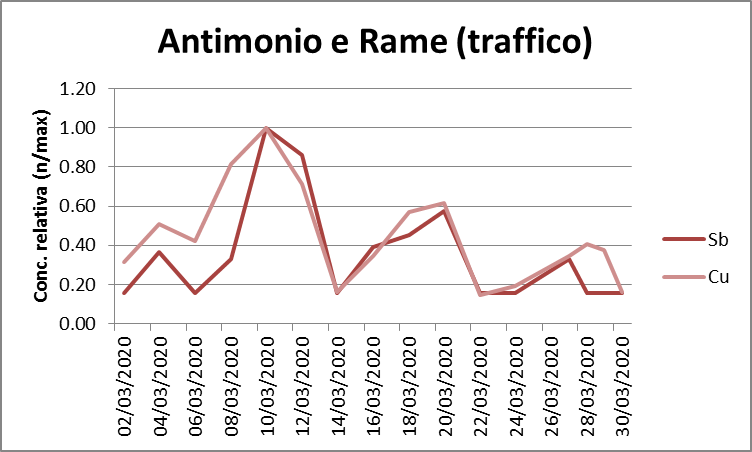
\includegraphics[width=0.45\textwidth]{figs/Sb-Cu-2020.png}
    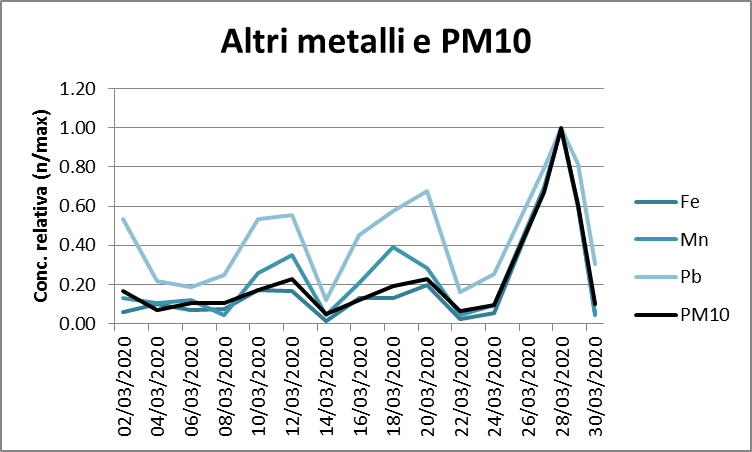
\includegraphics[width=0.45\textwidth]{figs/metalli-2020.png}\\
    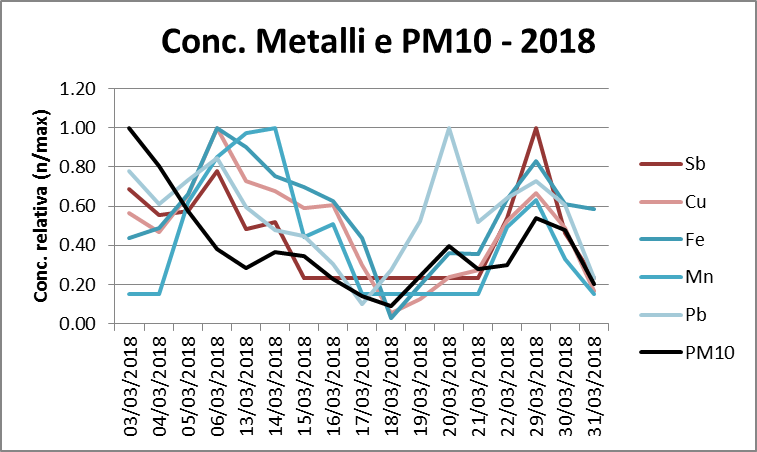
\includegraphics[width=0.45\textwidth]{figs/metalli-2018.png}
    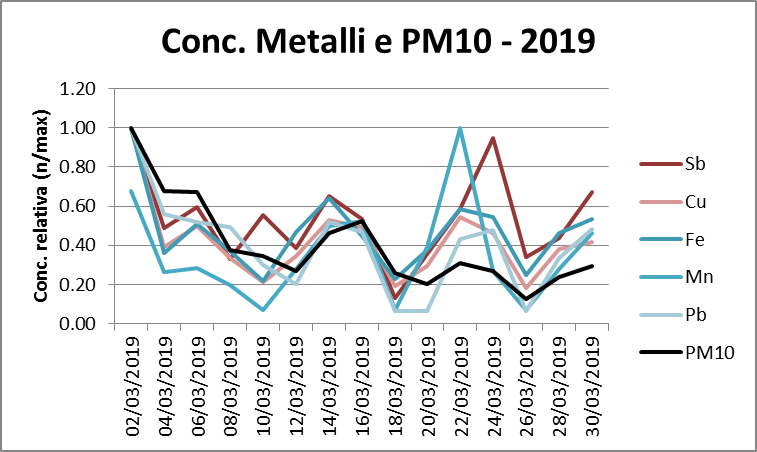
\includegraphics[width=0.45\textwidth]{figs/metalli-2019.png}
    \caption[Metalli nel PM10 a Udine]{Concentrazioni di metalli nel PM10, e del PM10 stesso, rilevate in marzo a Udine in via Cairoli e riscalate con il massimo del periodo. Sopra, a sinistra antimonio e rame, a destra ferro, manganese, piombo e PM10. Sotto, per confronto, a sinistra le concentrazioni degli stessi metalli nel marzo 2018, a destra nel marzo 2019.}
    \label{fig:metalli1}
\end{figure}

\begin{landscape}
\begin{figure}
    \centering
    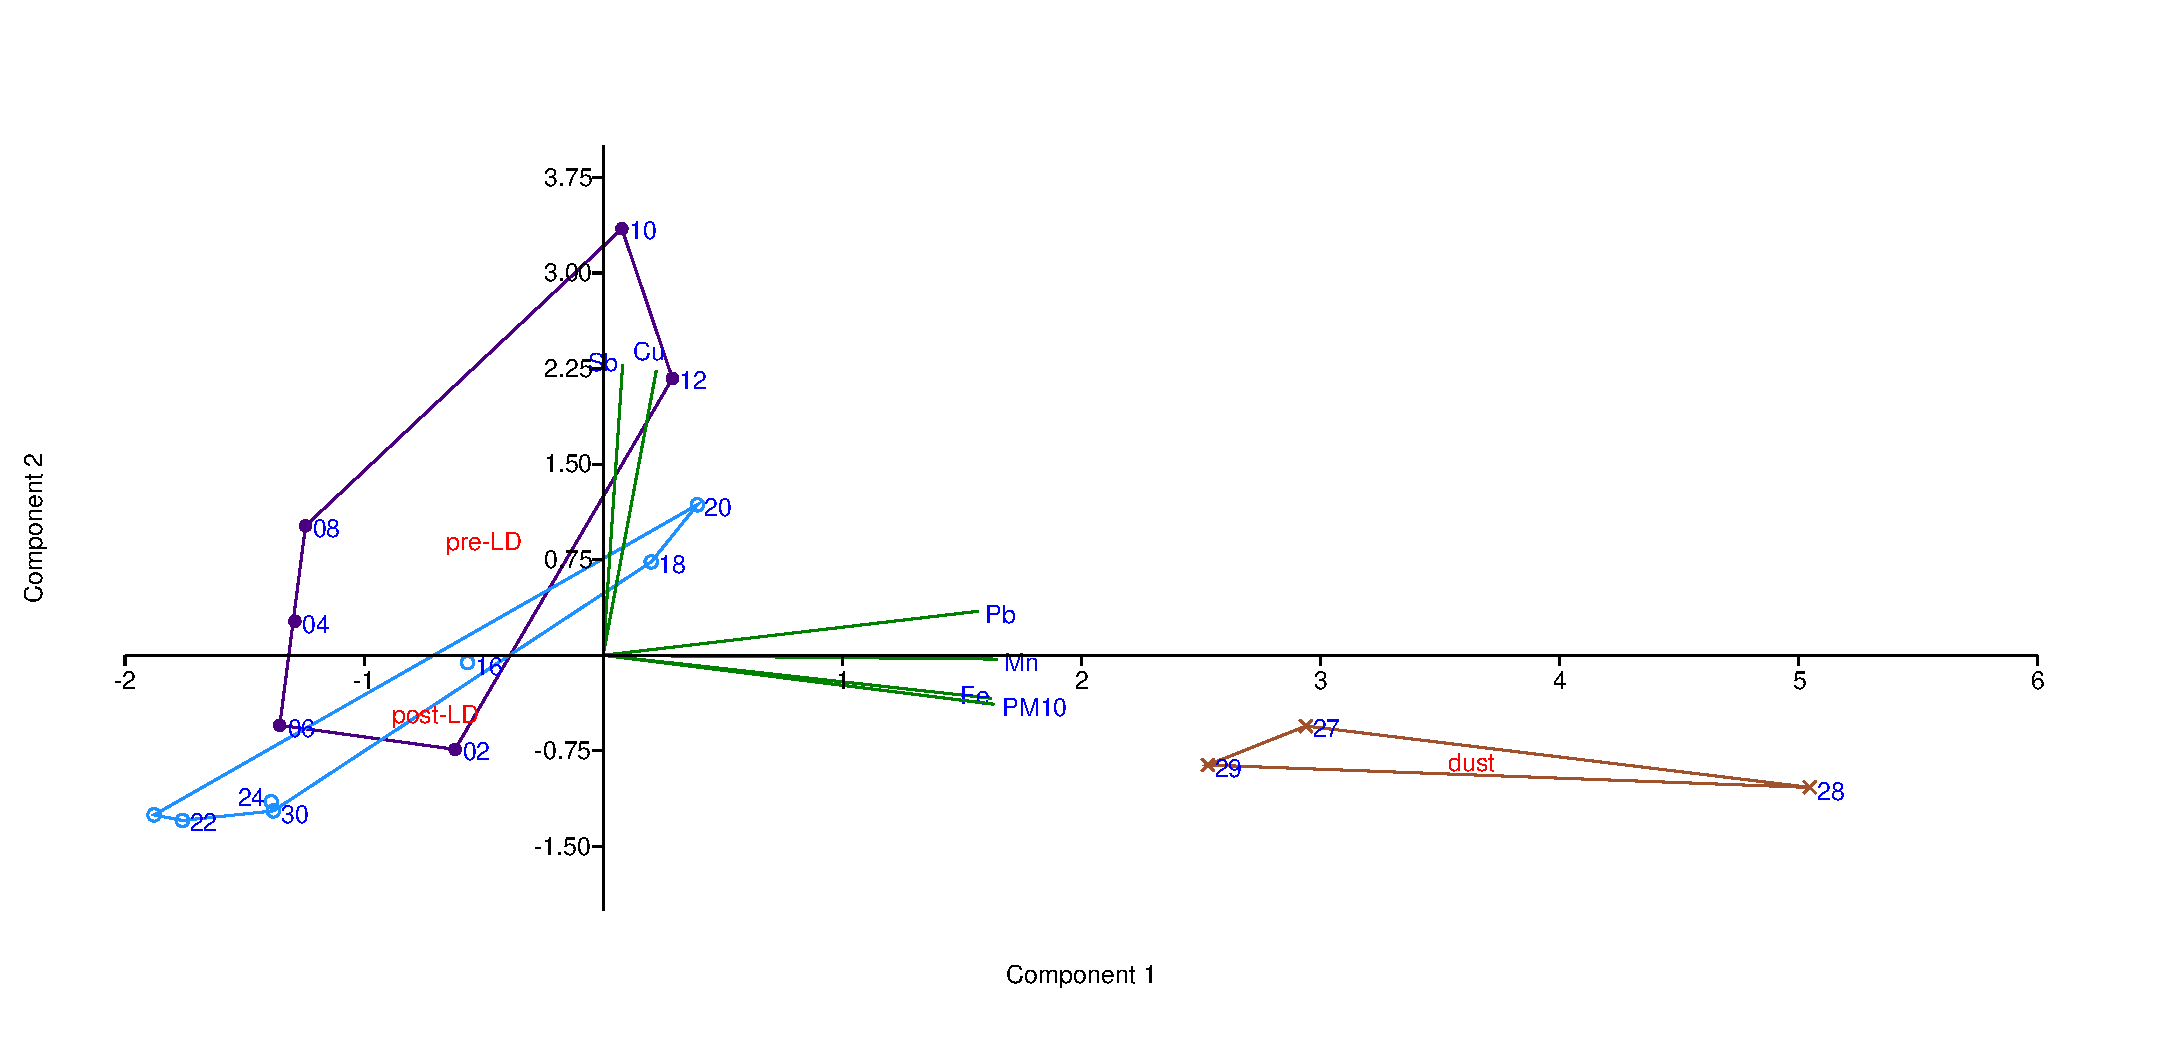
\includegraphics[width=0.9\linewidth]{figs/pca-metalli.pdf}
    \caption[PCA dei metalli nel PM10 a Udine]{Analisi delle componenti principali dei metalli nel PM10, rilevati nel marzo 2020 a Udine in via Cairoli. I numeri in blu identificano le date di campionamento. Le “X” marroni identificano i campioni raccolti nelle giornate di trasporto di polveri desertiche, i pallini viola i campioni pre-\textit{lockdown}, i cerchietti azzurri i campioni relativi al periodo di \textit{lockdown}. I vettori in verde rappresentano le proiezioni degli assi relativi alle variabili chimiche originali (\textit{loadings}).}
    \label{fig:metalli2}
\end{figure}
\end{landscape}


\FloatBarrier
\paragraph{Idrocarburi policiclici aromatici}\label{cap:ipa}
Gli idrocarburi policiclici aromatici (IPA) vengono comunemente ricercati nel PM10 data la loro tossicità; per uno di essi, il benzo(a)pirene (BaP), sussiste inoltre il limite legale di $1 ng/m^3$ come media annua. Questi inquinanti originano da processi di combustione fra cui si rammentano il traffico veicolare e il riscaldamento domestico. In regione sono molte le stazioni dedicate a questo tipo di indagine in quanto le medie annue di BaP risultano, ancorché entro il limite di $1 ng/m^3$, spesso al di sopra della soglia di valutazione superiore.

Sono state analizzate le concentrazioni degli IPA campionati in 3 stazioni in provincia di Udine: la stazione di fondo urbano di Udine centro (v. Cairoli), la stazione urbana di montagna di Tolmezzo e la stazione suburbana di montagna di Ugovizza. Essendo gli IPA una tipologia di inquinanti dovuta alla combustione, e di natura prevalentemente invernale (sia per la maggiore presenza di fonti di emissione come il riscaldamento domestico, sia per la natura chimica e fotochimica di questi composti), il mese di marzo registra solitamente concentrazioni abbastanza basse di questi analiti, spesso vicini al limite di rilevazione strumentale (LOQ). Per questo motivo, l’analisi viene effettuata su “cumuli” di filtri giornalieri, al fine di raggiungere in ciascuna analisi una quantità di inquinante analiticamente apprezzabile. I campioni del mese di marzo sono stati quindi “cumulati” su questi periodi: 
\begin{itemize}
    \item 1--13/3, prima del \textit{lockdown} (“tr ON” nei grafici);
    \item 14--26/3, durante il \textit{lockdown} (“tr OFF”);
    \item 27--29/3, durante l'evento di trasporto di polveri desertiche ("dust");
    \item 30--31/3 ("norm").
\end{itemize}

\begin{figure}
    \centering
    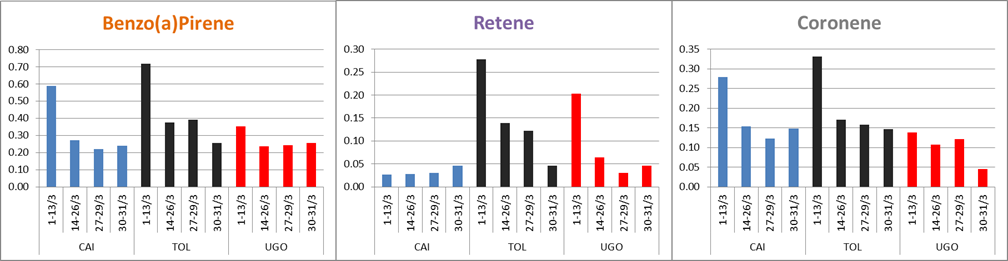
\includegraphics[width=\textwidth]{figs/ipa-barre.png}
    \caption[Concentrazioni in atmosfera di BaP, retene e coronene]{Concentrazioni in atmosfera (in $ng/m^3$) dei tre IPA benzo(a)pirene, retene e coronene, nei tre siti di Udine CAI, Tolmezzo TOL e Ugovizza UGO.}
    \label{fig:ipa2}
\end{figure}

Il \textit{lockdown} ha dunque impatti diversi sui tre IPA benzo(a)pirene, retene e coronene (fig.\ref{fig:ipa2}). Il confronto tra i primi 13 giorni del mese e le giornate seguenti lo evidenzia. Il retene (origine: combustione di legna resinosa) risulta sostanzialmente assente nella stazione urbana di Udine, mentre gli altri composti, ampiamente presenti nel sito, risentono del \textit{lockdown}. Le concentrazioni di benzo(a)pirene e coronene sono sostanzialmente dimezzate (rispetto ai primi 13 giorni del mese) in tutte le stazioni tranne quella di Ugovizza: in quest’ultima stazione l’entità del decremento è minore, a testimonianza del minore impatto della fonte traffico su quel sito.

\begin{figure}
    \centering
    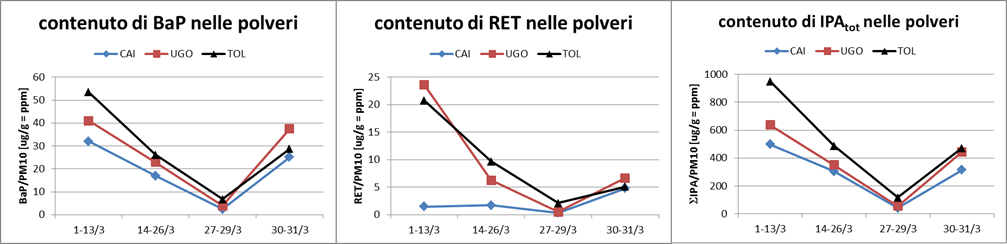
\includegraphics[width=\textwidth]{figs/ipa-linee.png}
    \caption[Concentrazioni nel PM10 di BaP, retene e IPA totali]{Concentrazioni nel PM10 di BaP, retene e IPA totali, nei tre siti di Udine CAI, Tolmezzo TOL e Ugovizza UGO.}
    \label{fig:ipa3}
\end{figure}

Se le sostanze aerodisperse vengono riferite, anziché al metro cubo d’aria, alla concentrazione di PM10 effettivamente presente in quello stesso metro cubo d’aria, si nota come il contenuto di BaP e di IPA totali nelle polveri (\ref{fig:ipa3}, primo e terzo pannello), diminuisce con il \textit{lockdown}, ed ancor più durante il successivo episodio di polveri desertiche. Nelle ultime giornate del mese, il contenuto di IPA torna a livelli del tutto simili a quelli del primo periodo di \textit{lockdown}.

\begin{figure}
    \centering
    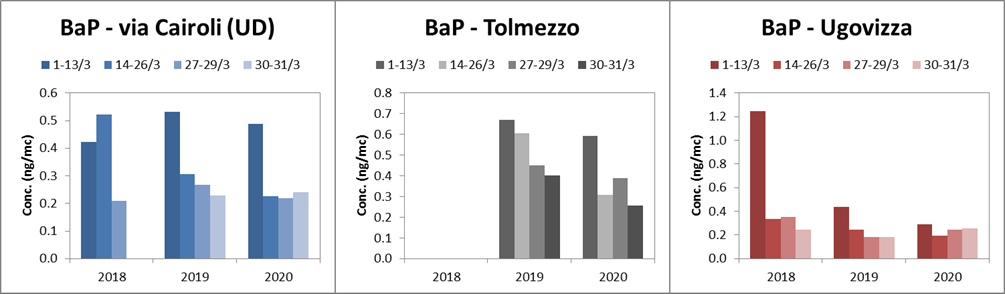
\includegraphics[width=\textwidth]{figs/bap-barre.png}
    \caption{Concentrazioni di BaP a marzo 2020, confronto con i due anni precedenti}
    \label{fig:ipa4}
\end{figure}
\begin{figure}
    \centering
    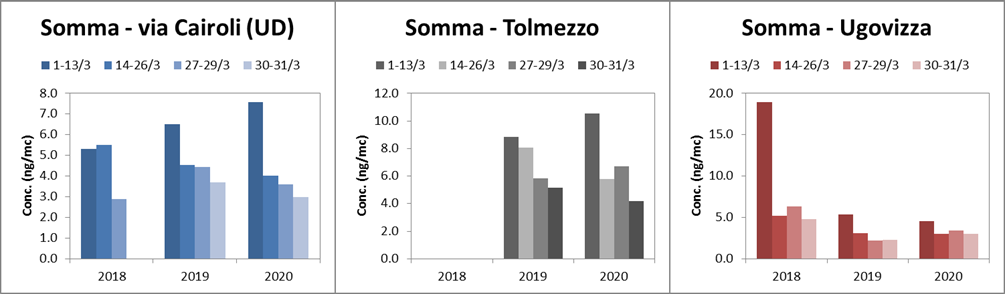
\includegraphics[width=\textwidth]{figs/ipa-somma-barre.png}
    \caption{Concentrazioni di IPA totali a marzo 2020, confronto con i due anni precedenti}
    \label{fig:ipa5}
\end{figure}

Come per altri inquinanti, la difficoltà nel trarre conclusioni definitive sugli effetti del \textit{lockdown} deriva dal fatto che esso si è verificato in un mese di transizione tra una stagione fredda e una più mite. Le figure \ref{fig:ipa4} e \ref{fig:ipa5} evidenziano come anche nei due anni precedenti si sia registrata una netta variazione nell'arco del mese. Tuttavia, nella stazione di Udine la variazione è stata decisamente più marcata che in passato. Ciò suggerisce che il \textit{lockdown} abbia avuto un impatto sugli IPA più marcato nelle aree maggiormente urbanizzate.

Per superare in qualche misura le limitazioni di queste analisi univariate, si è realizzata un'analisi multivariata, tenendo in considerazione contemporaneamente tutti i congeneri IPA analizzati. Si è condotta un’Analisi delle Componenti Principali PCA, \citep{wold1984multivariate}, riportando nel piano delle prime due Componenti Principali sia la proiezione dei campioni che quella delle variabili chimiche originali: si ottiene cioè il \textit{biplot}\footnote{varianza spiegata dal biplot: 92\%, di cui varianza spiegata dalla prima componente principale (PC1, asse orizzontale): 83\%; varianza spiegata dalla PC2 (asse verticale): 10\%.} riportato in figura \ref{fig:ipa1}.

Poiché i \textit{loadings} di quasi tutti i congeneri IPA sono orientati verso i due quadranti di destra (cioè sul verso positivo della PC1), mentre quello del retene (“RET” nel grafico\footnote{il retene è un alchil-IPA derivante dalla combustione dell’acido abietico contenuto nelle resine delle conifere}), risulta orientato verso il basso, a differenza della maggior parte degli altri congeneri, è possibile identificare la PC1 (asse orizzontale) come una componente che rendiconta la generale intensità dell’impatto degli IPA, e la PC2 come una componente che discrimina tra la fonte traffico e la fonte da combustione di biomassa (\textit{biomass burning}). 
Dunque i campioni a maggior impatto complessivo da IPA si collocano a destra nel grafico, quelli a minor impatto da IPA a sinistra; i campioni a prevalente fonte traffico si collocano in alto, mentre quelli a prevalente fonte \textit{biomass burning} si collocano in basso.

La transizione dal periodo pre-\textit{lockdown} ("tr ON" nel \textit{biplot}) al periodo di \textit{lockdown} ("tr OFF") è differente per le tre stazioni: 
\begin{itemize}
    \item a Udine si registra un netto spostamento dalla zona ad alto impatto di IPA di origine traffico a quella a basso impatto di IPA; 
    \item anche a Tolmezzo il \textit{lockdown} determina una netta attenuazione dell'impatto da IPA, ma rispetto a Udine il contributo della combustione di legna è più marcato, e durante il blocco risulta prevalente;
    \item infine a Ugovizza l'impatto degli IPA è molto minore, soprattutto ascrivibile alla combustione di biomassa legnosa, e non significativamente alterato dal \textit{lockdown}.
\end{itemize}

\begin{landscape}
\begin{figure}
    \centering
    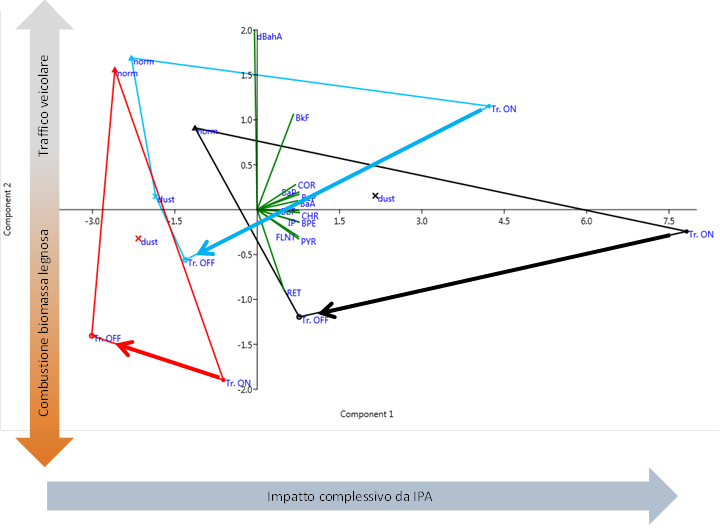
\includegraphics[width=0.9\linewidth]{figs/ipa-pca.png}
    \caption[PCA degli IPA a Udine, Tolmezzo e Ugovizza]{PCA degli IPA a Udine (azzurro), Tolmezzo (nero) e Ugovizza (rosso). I vettori in verde rappresentano le proiezioni degli assi relativi alle variabili chimiche originali (\textit{loadings}). Le etichette blu individuano i quattro periodi di campionamento: "tr ON" 1--13/3, "tr OFF" 14--26/3, "dust" 27--29/3, "norm" 30--31/3. Le frecce più spesse individuano la transizione da pre-\textit{lockdown} a \textit{lockdown}.}
    \label{fig:ipa1}
\end{figure}
\end{landscape}


%\section{Approfondimenti}
%\subsection{Trasporto a grande distanza di polveri desertiche}
%\subsection{Concentrazioni attese in assenza di azioni di contenimento}

\FloatBarrier\pagebreak
\section*{Conclusioni}
\addcontentsline{toc}{section}{Conclusioni}
I provvedimenti di confinamento e di limitazione della mobilità, messi in atto a livello locale, regionale e nazionale (tab.\ref{tab:cronistoria}) per contenere il contagio di COVID-19, hanno determinato alcuni effetti sulla matrice ambientale aria.

I flussi di traffico sono diminuiti progressivamente (fig.\ref{fig:riduzionedeterminanti}) a partire dalla quarta settimana di febbraio, fino a raggiungere nelle ultime settimane di marzo riduzioni - rispetto alle condizioni normali - nelle aree urbane di oltre il 70\%, sulle strade extraurbane e autostrade di oltre l'80\% dei veicoli leggeri e del 50-70\% dei veicoli pesanti.
Nel frattempo, anche il traffico aereo è stato drasticamente ridotto  (fig.\ref{fig:riduzionedeterminanti}), fino ad azzerarsi nelle ultime settimane di marzo. Le variazioni delle attività industriali e portuali e dei consumi energetici per il riscaldamento domestico saranno oggetto di ulteriori approfondimenti.

Riduzioni così marcate di alcune attività antropiche hanno determinato flessioni significative nelle emissioni di alcuni inquinanti  (fig.\ref{fig:riduzioneemissioni}), stimate tenendo conto delle riduzioni di traffico stradale e aereo nell'ordine del 25\% per gli ossidi di azoto, del 19\% per l'anidride carbonica, del 16\% per il monossido di carbonio. Decisamente minori sono risultate le riduzioni delle emissioni dei composti organici volatili (circa -4\%), dell'ammoniaca (-3\%) e di polveri sottili (circa -8\%). L'entità di queste riduzioni è coerente con il fatto che le misure adottate nella nostra regione hanno agito soprattutto sui trasporti. Il probabile aumento dei consumi per il riscaldamento domestico potrebbe però aver parzialmente compensato la riduzione di emissioni di polveri sottili.

La riduzione delle emissioni inquinanti ha determinato un calo delle concentrazioni di biossido di azoto (circa -40\% rispetto agli anni precedenti), registrato dalle stazioni di monitoraggio regionali, che sostanzialmente ha anticipato di tre o quattro settimane la consueta diminuzione delle concentrazioni che si osserva in primavera  (figg.\ref{fig:andaminq} e \ref{fig:giornino2}). Tale riduzione è ascrivibile alle azioni di contenimento, poiché si manifesta attraverso una brusca attenuazione dei picchi corrispondenti alle ore di punta del traffico  (fig.\ref{fig:noxgiorni}), ma ad essa hanno anche contribuito le condizioni di vivace ventilazione, specie nell'area triestina  (figg.\ref{fig:RSV} e \ref{fig:giornivento}). Altrettanto rilevante, nelle postazioni per il monitoraggio degli impatti del traffico, è stato il calo delle concentrazioni di benzene, che si aggiunge alla diminuzione già osservata negli ultimi anni per questo inquinante  (figg.\ref{fig:andaminq} e \ref{fig:giornibenzene}).

Le polveri sottili hanno presentato un calo decisamente meno rilevante (pari o inferiore al 10\%) e fluttuazioni più marcate, determinate dalla meteorologia e da un evento di trasporto di polveri desertiche tra il 27 e il 29 marzo (figg.\ref{fig:andaminq} e \ref{fig:giornipm10}). 

L'ozono - inquinante fortemente legato alla radiazione solare e dunque molto variabile tra un anno e l'altro - non ha mostrato variazioni rilevanti rispetto agli anni precedenti, ma l'aumento delle concentrazioni in aprile potrebbe essere stato favorito in parte dalle azioni di contenimento  (figg.\ref{fig:andaminq} e \ref{fig:giornio3}). 

L'analisi condotta sui rapporti tra le concentrazioni di inquinanti ha consentito di ridurre l'effetto confondente della meteorologia e ha messo così in luce alcuni fenomeni interessanti. Il rapporto toluene/benzene - buon indicatore dell'origine prevalente delle emissioni locali di questi composti organici volatili - nelle settimane della serrata è calato vistosamente, seppur con ampie fluttuazioni, da valori tipici del traffico veicolare a valori caratteristici della combustione di legna (pag.\pageref{cap:tb} e sgg.). A fine aprile - in corrispondenza del mitigarsi delle temperature e dell'allentarsi delle misure di contenimento - tale indicatore è tornato a livelli più consueti. L'analisi del rapporto NOx/NO - il cui valore dipende sia dalla distanza delle fonti emissive sia dalla cinetica chimica - mostra che per gli ossidi di azoto gli effetti del \textit{lockdown} si sono manifestati soprattutto in prossimità delle strade  (pag.\pageref{cap:noxno} e sgg.). Analogamente, l'analisi granulometrica delle polveri sottili evidenzia il venir meno durante la serrata della risospensione di polveri grossolane, indotta dal transito di veicoli e usualmente registrata dalle stazioni di bordo strada (pag.\pageref{cap:cef} e sgg.).

L'analisi del contenuto di alcuni metalli nelle polveri sottili campionate a Udine, presenti in basse concentrazioni già prima dell'entrata in vigore delle azioni di contenimento, evidenzia un significativo calo di antimonio e rame, originati prevalentemente dall'usura dei freni dei veicoli, e conferma l'origine terrigena (deserti asiatici) delle notevoli masse di PM10 che hanno interessato tutta la regione tra il 27 e il 29 marzo (pag.\pageref{cap:metalli} e sgg.).

Anche sul contenuto di idrocarburi policiclici aromatici (IPA) nel PM10 le azioni di contenimento del contagio hanno determinato effetti misurabili. Agendo in particolare sul traffico, hanno determinato la riduzione degli IPA associati ai trasporti, facendo così risaltare quelli principalmente legati alla combustione domestica (pag.\pageref{cap:ipa} e sgg.).

\paragraph{Prospettive}
L'analisi degli effetti del \textit{lockdown} sulla matrice aria richiederà ulteriori approfondimenti ed estensioni temporali nei prossimi mesi, quando saranno disponibili più dati e sarà possibile valutare anche gli effetti della ripresa di molte attività.

La necessità di individuare i nessi causali tra riduzioni emissive ed effetti sulle concentrazioni in aria ha richiesto l'acquisizione tempestiva di informazioni sulle attività antropiche di interesse, l'elaborazione di specifici indicatori e l'uso di strumenti di analisi multi-variata. Tali flussi di dati e metodiche di analisi hanno rivelato un notevole potenziale a supporto dell'interpretazione dei fenomeni in atto. Pertanto si auspica lo sviluppo di collaborazioni e competenze in tal senso, che in futuro potrebbero rivelarsi fondamentali per valutare gli effetti di azioni strutturali e pianificate per il miglioramento della qualità dell'aria.

Lo studio ha evidenziato che la riduzione delle emissioni dei trasporti porta evidenti benefici ambientali, ma per alcuni inquinanti non è sufficiente, neppure se applicata su grande scala e per lungo tempo. Per il miglioramento della qualità dell'aria è necessario continuare ad intervenire anche su altri settori, quali il riscaldamento domestico, l'agricoltura e l'industria.  



\FloatBarrier\pagebreak
\section*{Glossario}
\addcontentsline{toc}{section}{Glossario}
\begin{tabular}{ll}
     BaP            & benzo(a)pirene\\
     CEF            & \textit{coarse enrichment factor}\\
     CO             & monossido di carbonio \\
     CO\textsubscript{2}& anidride carbonica \\
     CO\textsubscript{2 eq}& emissioni climalteranti totali espresse come equivalenti di anidride carbonica \\
     COV            & composti organici volatili\\
     COVID-19       & malattia respiratoria acuta da SARS-CoV-2 \\
     C\textsubscript{6}H\textsubscript{6}& benzene \\
     C\textsubscript{7}H\textsubscript{8}& toluene \\
     Cu             & rame\\
     DPSIR          & schema determinanti-pressioni-stato-impatti-risposte\\
     Fe             & ferro\\
     FVG            & Friuli Venezia Giulia\\
     IPA            & idrocarburi policiclici aromatici\\
     OMS            & Organizzazione Mondiale della Sanità\\
     Mn             & manganese\\
     NO\textsubscript{x}& ossidi di azoto \\
     NO\textsubscript{2}& biossido di azoto \\
     O\textsubscript{3}& ozono \\
     Pb             & piombo\\
     PCA            & analisi delle componenti principali\\
     PM10           & materiale particolato aerodisperso con diametro aerodinamico inferiore ai 10 micron\\
     PM2.5          & materiale particolato aerodisperso con diametro aerodinamico inferiore ai 2.5 micron\\
     RAFVG          & Regione Autonoma Friuli Venezia Giulia\\
     SARS-CoV-2     & coronavirus 2 da sindrome respiratoria acuta grave \\
     Sb             & antimonio\\
     SO\textsubscript{2}& biossido di zolfo \\
\end{tabular}


\FloatBarrier\pagebreak
\bibliography{biblio}
\bibliographystyle{apalike}

\end{document}
